\documentclass[11pt]{article}
\usepackage[margin=1in]{geometry}
\usepackage[T1]{fontenc}
\usepackage[utf8]{inputenc}
\usepackage{lmodern}
\usepackage{microtype}
\usepackage{amsmath,amssymb}
\usepackage{graphicx}
\usepackage{booktabs,tabularx,array}
\usepackage{float}
\usepackage[section]{placeins}
\usepackage{rotating}
\usepackage[font=small,labelfont=bf]{caption}
\usepackage{enumitem}
\usepackage[hidelinks]{hyperref}

\setlist{itemsep=2pt,topsep=4pt}
\providecommand{\tightlist}{\setlength{\itemsep}{2pt}\setlength{\parskip}{0pt}}
\newcommand{\source}[1]{\par\vspace{3pt}{\footnotesize\textit{Source:} #1\par}}
\newcommand{\tablenote}[1]{\par\vspace{3pt}{\footnotesize #1\par}}
% a table is scaled down only if it is wider than the text block
\newsavebox{\fitbox}
\newcommand{\fittable}[1]{\sbox{\fitbox}{\input{#1}}%
  \ifdim\wd\fitbox>\textwidth\resizebox{\textwidth}{!}{\usebox{\fitbox}}\else\usebox{\fitbox}\fi}
\newenvironment{reflist}{\begin{list}{}{\setlength{\leftmargin}{1.5em}\setlength{\itemindent}{-1.5em}\setlength{\itemsep}{3pt}\setlength{\parsep}{0pt}}}{\end{list}}
\renewcommand{\arraystretch}{1.12}

\title{Does Machine Learning Add Selection Skill to a Trend Strategy?\\[6pt]
\large A Ridge market-state filter and momentum stock selection on a moving-average rule}
\author{Sixian Li \and Tai Karir \and Zizhao Ding}
\date{MATH 628, Machine Learning for Finance I\\ Final project report, Fall 2026}

\begin{document}
\maketitle

\begin{abstract}
\noindent A dual moving-average rule keeps an investor out of long bear markets, but it stays invested through sharp declines inside an uptrend. We ask whether a machine-learning model can tell the rule which of its invested weeks to skip.

Our first design, the one in our project proposal, was a classifier (logistic regression, random forest, gradient boosting) that predicts the direction of next week's return from seven price features. It has no predictive skill: test AUC is between 0.49 and 0.54, and the classifiers keep 99\% or more of the rule's weeks. We trace the failure to the prediction target and to the information set, and we redesign the filter as a Ridge regression that forecasts the size of next week's return from 16 market-state features: implied volatility, the breadth of the Nasdaq-100 members, and cross-asset strength.

On QQQ with an SMA20/140 rule, in an annual walk-forward over 2005--2025, the redesigned filter earns the rule's total return while invested in 51\% of the weeks instead of 79\%. The return per year invested (holding CAGR) rises from 14.3\% to 22.7\%, and from 23.2\% to 33.4\% in 2019--2025, a period we held out. Holding the ten Nasdaq-100 stocks with the highest 12-month return in the weeks the filter keeps turns this into a higher total return: 19.1\% a year over 2005--2025 with a Sharpe ratio of 1.07 and a maximum drawdown of about 27\%, against 14.8\%, 0.77 and 52\% for buying and holding QQQ. In an ablation over 2005--2025, removing any one of the three components (trend rule, Ridge filter, momentum ranking) lowers both the Sharpe ratio and the holding CAGR.

The gain is concentrated in periods that contain bear markets. In rising markets the strategy's total return is about equal to that of a momentum portfolio that is always invested, and in one of four test periods (2013--2018) it is lower.
\end{abstract}

\section{Background}

\subsection{Trend following with two moving averages}

A simple moving average (SMA) of length \(n\) is the mean of the last \(n\) daily closing prices. A dual-SMA rule compares a short average with a long one and holds the asset only while the short average is above the long one. We use 20 and 140 trading days throughout and write the rule as SMA20/140. The rule is checked once a week: the signal is read at the last close of the week, and the position is changed at the next open.

The rule is a risk control. It leaves the market some time after a decline has started and comes back some time after a recovery has started, so it avoids most of a long bear market and gives up part of every rebound. Figure 1 shows both effects on QQQ, the exchange-traded fund that tracks the Nasdaq-100 index. From 2005 to 2025, buying and holding QQQ earned 14.8\% a year with a maximum drawdown of 52\%. The SMA20/140 rule earned 11.1\% a year with a maximum drawdown of 31\%, and it was invested in 79\% of the weeks.

\begin{figure}[!htbp]
\centering
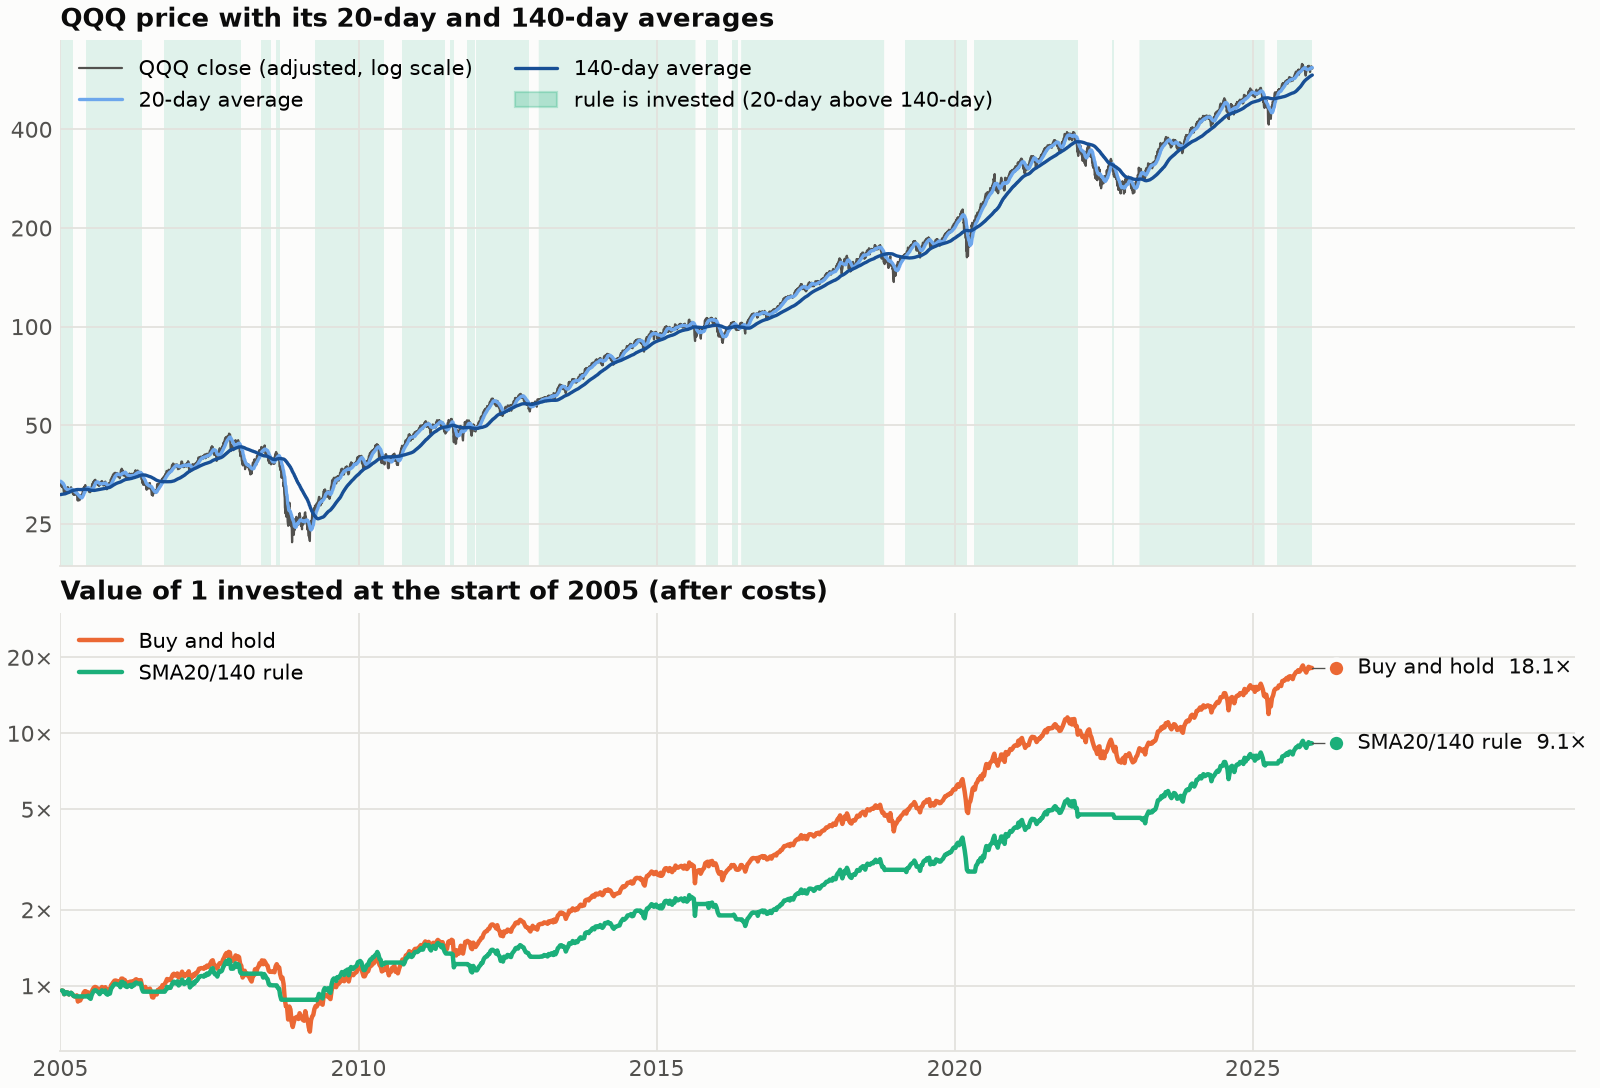
\includegraphics[width=\textwidth]{figures/fig1_qqq_rule.png}
\caption{Top: QQQ with its 20-day and 140-day moving averages, 2005--2025; shaded periods are those in which the SMA20/140 rule is invested. Bottom: buy-and-hold against the rule, after costs of 5 basis points per trade. The rule avoids most of the 2008 and 2022 declines and ends with about half of the buy-and-hold wealth.}
\label{fig:qqq-rule}
\source{\texttt{reports/exhibits/qqq\_daily.csv}, \texttt{equity\_weekly.csv}}
\end{figure}

\subsection{What the rule cannot see}

The rule looks only at two averages of past prices, so it reacts slowly by construction. Figure 2 shows what that means in one short episode. In the summer of 2025 Palantir (PLTR) was in a strong uptrend, with its 20-day average far above its 140-day average. Its close peaked at 186.97 on 12 August. Six trading days later it stood at 156.01, a drop of 16.6\%, and on 2 September the stock opened at 151.20. The two averages never came close to crossing, so a dual-SMA rule on the stock stayed fully invested through the whole decline.

\begin{figure}[!htbp]
\centering
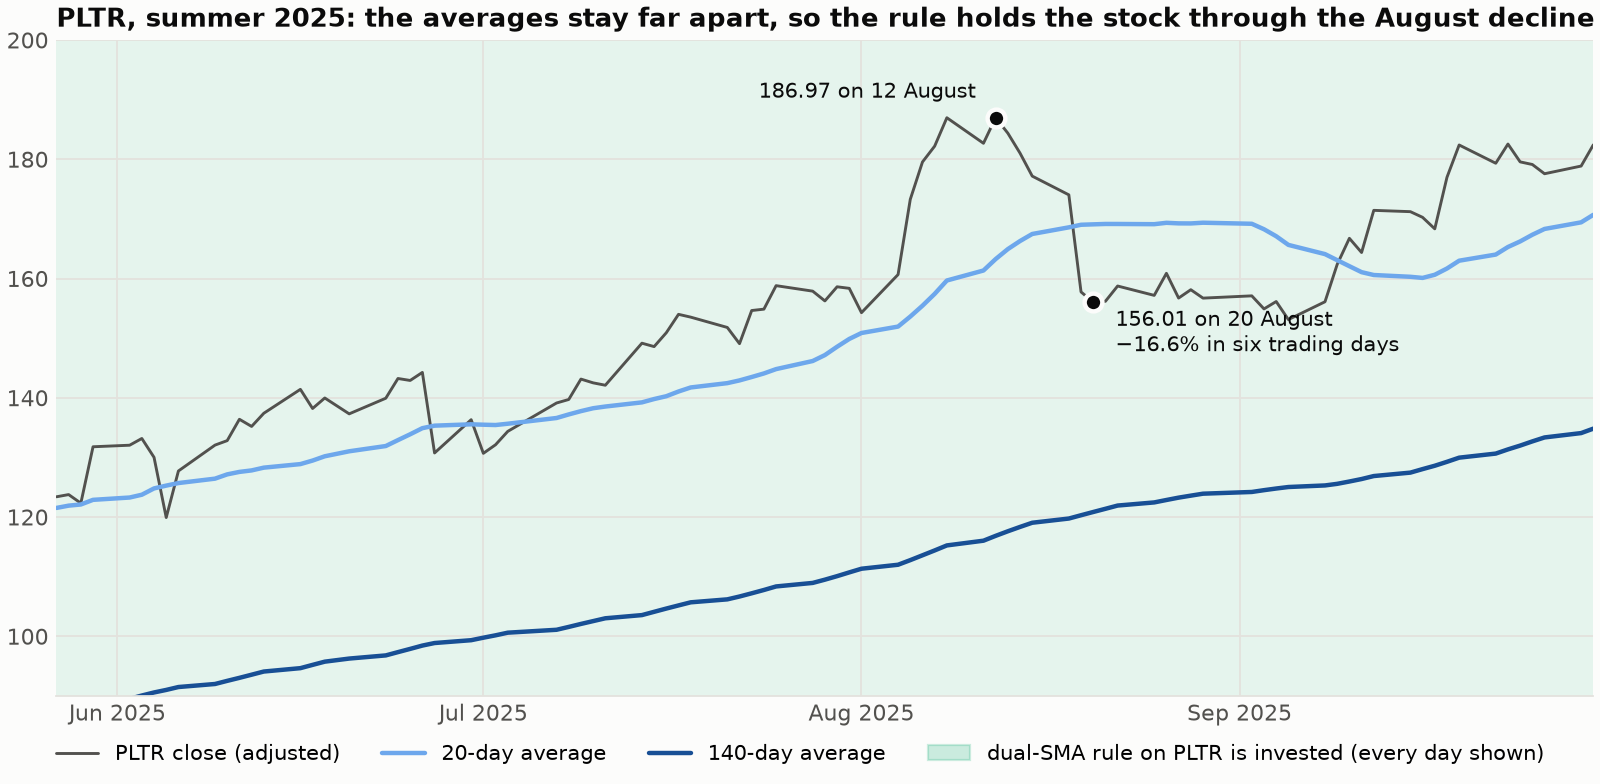
\includegraphics[width=0.95\textwidth]{figures/fig2_example_rule.png}
\caption{PLTR from late May to September 2025 with its 20-day and 140-day averages. The 20-day average is above the 140-day average on every day shown, so the dual-SMA rule is invested throughout and sits through the August decline.}
\label{fig:example-rule}
\source{\texttt{reports/exhibits/example\_daily.csv}}
\end{figure}

Shorter windows would react faster, but they also leave the market on small dips and come back later at a higher price. Our question keeps the rule as it is and adds a second signal: one that says when to step aside although the rule still says ``in''. A signal that said ``sell'' in the second week of August would have avoided the decline. We return to this example in Section 7.3 and show what our filter did.

\subsection{When to be invested, and what to hold}

The project has three parts, and each answers a different question.

\begin{enumerate}
\def\labelenumi{\arabic{enumi}.}
\tightlist
\item
  \textbf{The SMA rule} decides when the market may be held at all.
\item
  \textbf{A machine-learning filter} decides which of those weeks to keep. This is where the methods of the course are used.
\item
  \textbf{A momentum ranking} decides what to hold in the weeks that are kept: the index fund, or the ten Nasdaq-100 stocks with the highest return over the past 12 months.
\end{enumerate}

\subsection{How a filter should be measured}

A filter can only remove invested weeks. In a rising market this lowers total return almost mechanically, so total return alone cannot separate a useful filter from a useless one. We report the following numbers side by side.

\begin{itemize}
\tightlist
\item
  \textbf{CAGR}: compound annual growth rate over calendar time, \((V_T/V_0)^{1/\text{years}} - 1\).
\item
  \textbf{Exposure}: the share of weeks in which the strategy is invested.
\item
  \textbf{Holding CAGR}: growth per year actually spent in the market, \((V_T/V_0)^{52/N} - 1\), where \(N\) is the number of invested weeks.
\item
  \textbf{Sharpe ratio}: mean weekly return divided by its standard deviation, times \(\sqrt{52}\), with a cash rate of zero.
\item
  \textbf{Maximum drawdown}: the largest loss from a previous peak, measured at weekly marks.
\end{itemize}

A filter that drops weeks at random leaves holding CAGR unchanged on average and lowers CAGR. A filter with skill raises holding CAGR. Holding CAGR has a known weakness: when few weeks are invested it is computed from a short history and becomes large and unstable. We therefore always show it next to exposure, and we read it as a measure of selection. Idle cash earns zero in all our tests, so holding CAGR is not a return an investor receives.

\subsection{Summary of findings}

\begin{itemize}
\tightlist
\item
  The filter in our proposal, a classifier of next week's direction built on price features, has no skill (Section 5).
\item
  Three things were wrong with it: the target, the information set, and the direction of what it could learn. A filter that changes all three raises the SMA rule's holding CAGR from 14.3\% to 22.7\% over 2005--2025 at an unchanged total return (Sections 6, 7.1 and 7.2).
\item
  Adding momentum stock selection raises total return to 19.1\% a year with a Sharpe ratio of 1.07 and a maximum drawdown of about 27\%. Over 2005--2025, removing any one of the three components lowers the Sharpe ratio and the holding CAGR (Section 7.3).
\item
  The result holds for most of 222 moving-average pairs, in a test that runs backwards in time, and in a leave-one-period-out test. It is strongest in periods with bear markets and weakest in 2013--2018 (Section 7.4).
\item
  In rising markets the strategy does not beat an always-invested momentum portfolio on total return (Section 7.5).
\end{itemize}

\section{Literature review}

\textbf{Trend rules.} Brock, Lakonishok and LeBaron (1992) test moving-average and trading-range rules on the Dow Jones index from 1897 to 1986 and find that buy signals are followed by higher returns than sell signals. Sullivan, Timmermann and White (1999) re-examine these rules with a bootstrap that accounts for the search over a large set of rules, the data-snooping problem. Faber (2007) uses a 10-month moving average as a timing rule and reports equity-like returns with much lower volatility and drawdown, which is how we use the SMA rule. Moskowitz, Ooi and Pedersen (2012) document time-series momentum, an asset's own past return predicting its future return, in each of 58 liquid instruments across equity index, currency, commodity and bond futures. We take two things from this work: a trend rule is a risk control, and its parameters are easy to overfit. For the second reason we repeat our tests over 222 moving-average pairs.

\textbf{Momentum across stocks.} Jegadeesh and Titman (1993) show that buying stocks that have performed well and selling stocks that have performed poorly earns significant returns over holding periods of 3 to 12 months. Daniel and Moskowitz (2016) show that momentum portfolios suffer large losses in ``panic'' states, after market declines and when volatility is high, and that these crashes are partly forecastable. This is the reason to hold a momentum portfolio only when a market-level signal allows it.

\textbf{Machine learning as a trade filter.} López de Prado (2018) describes meta-labeling: a primary rule proposes trades and a secondary model decides whether to take them (see also Joubert, 2022). Our first design has this structure. Gu, Kelly and Xiu (2020) find that trees and neural networks give the best return forecasts on a large panel of U.S. stocks. Israel, Kelly and Moskowitz (2020) point out that return prediction is a small-data, low signal-to-noise problem, which limits flexible models. Welch and Goyal (2008) find that most published predictors of the equity premium fail out of sample, so a negative result is the outcome to expect. Christoffersen and Diebold (2006) show that volatility dynamics alone make the \emph{sign} of a return predictable: with a positive expected return, the higher the volatility, the lower the probability of a positive return. We use this to explain why a direction classifier behaves like a volatility filter.

\textbf{Market state.} Bollerslev, Tauchen and Zhou (2009) show that the gap between implied and realized variance predicts aggregate stock returns, with a wide gap followed by high returns. Nagel (2012) finds that the return to providing liquidity rises sharply with the VIX. Moreira and Muir (2017) argue for the opposite action, cutting exposure when volatility is high; Cederburg, O'Doherty, Wang and Yan (2020) find that real-time versions of such strategies do not systematically beat the unmanaged portfolios. Market breadth, the balance of rising over falling stocks, predicts the returns of market and industry portfolios in 64 countries in Zaremba, Szyszka, Karathanasopoulos and Mikutowski (2021). Yu, Webb and Lin (2025) test breadth ratios and the share of an index above its moving averages, and conclude that some of these indicators may help to predict market movements. Neely, Rapach, Tu and Zhou (2014) show that technical indicators and macroeconomic variables carry complementary information. The evidence on what to do when volatility is high is therefore mixed, and it suggests that information outside the price series can add to a technical rule.

\textbf{Backtest overfitting.} Bailey, Borwein, López de Prado and Zhu (2014) show how easily a good backtest is produced by trying many configurations. Harvey, Liu and Zhu (2016) argue that, after decades of data mining, a newly proposed factor should clear a \(t\)-statistic of 3.

\textbf{The gap.} These strands are mostly studied one at a time: trend rules on their own, classifiers as filters on generic signals, volatility timing on factor portfolios. We put a trend rule, a machine-learning filter and a momentum ranking on one account with the same timing and costs, and we measure what each adds to the others.

\section{Our contribution}

\begin{enumerate}
\def\labelenumi{\arabic{enumi}.}
\tightlist
\item
  \textbf{A way to judge a filter.} We evaluate a filter by holding CAGR together with exposure, and we test it against a placebo that keeps how often and how persistently the filter steps aside (Sections 1.4 and 7.1).
\item
  \textbf{A diagnosis of why the standard design fails.} We show with data why a direction classifier on price features cannot improve the trend rule, and we separate the two causes in a 2$\times$2 comparison of features and targets (Sections 5.3 and 7.2).
\item
  \textbf{A redesigned filter.} Sixteen market-state features, the size of the return as the target, and a Ridge regression. We report one configuration fixed in advance of the 2019--2025 results and the family of 45 configurations around it (Sections 6, 7.1 and 7.2).
\item
  \textbf{A three-component strategy with a full ablation.} Trend rule, Ridge filter and momentum ranking, with all eight on/off combinations on one account (Section 7.3).
\item
  \textbf{Robustness tests reported with their weak spots.} The strategy over 222 moving-average pairs, a test that fits on late years and applies to early ones, a leave-one-period-out test, and a list of what does not hold (Sections 7.4 and 7.5).
\end{enumerate}

\section{Data and conventions}

\begin{table}[H]
\centering\small
\caption{Data.}
\label{tab:data}
\begin{tabularx}{\textwidth}{@{}p{0.27\textwidth}Xp{0.27\textwidth}@{}}
\toprule
Data & Content & Used for \\
\midrule
QQQ daily bars, 1999--2025 & Split- and dividend-adjusted open and close, from a commercial vendor (Rethink) & The trend rule, the filter's target, the QQQ strategies \\
\addlinespace
Nasdaq-100 point-in-time members & 480 securities, including delisted names: adjusted daily bars and a daily in-index flag, same vendor & Breadth features and the stock portfolios \\
\addlinespace
VIX & Cboe volatility index, daily & Volatility features \\
\addlinespace
SPY, IWM and nine sector ETFs & Adjusted daily closes, same vendor & Cross-asset features \\
\bottomrule
\end{tabularx}
\end{table}

The sample is 2000--2025, with 1999 used to initialize the moving averages. The following conventions apply to every result.

\begin{itemize}
\tightlist
\item
  \textbf{Timing.} Features and signals use the last close of the week. Trades are filled at the open of the next session. The weekly return \(R_t\) runs from that open to the open one week later.
\item
  \textbf{Costs.} Five basis points per side on every change in weight, including moving a whole stock portfolio in and out of the market. Cash earns zero.
\item
  \textbf{Stock data.} Index membership is taken one session before each decision, so a stock is used only while it was actually in the index. A holding that is delisted is settled at its last close.
\item
  \textbf{One account for all strategy tables.} Tables 6 and 10--15 use the same weekly account. Tables 2, 7 and 8 and the diagnostics quoted in Section 7.1 (placebo, costs, yearly comparison) come from a single-asset account that is marked daily; its numbers differ from the weekly account in the first decimal.
\item
  \textbf{A data limit.} The stock package is a vendor candidate with open quality flags (742 flagged daily moves, none removed). Results that use individual stocks should be read as indicative.
\end{itemize}

\section{Methodology I: a direction classifier, and why it failed}

\subsection{Design}

The first design follows the meta-labeling idea: the SMA rule proposes the weeks to be invested, and a classifier accepts or rejects each one.

\begin{itemize}
\tightlist
\item
  \textbf{Target.} For each week \(t\) in which the rule is invested, the label is the direction of the next weekly return, \(y_t = \mathbf{1}\{R_t > 0\}\).
\item
  \textbf{Features.} Seven numbers computed from QQQ's own price: the 5-day and 20-day returns, the gap between the 20-day and 60-day averages, the gap between the price and the 20-day average, the 5-day change of the 60-day average, 20-day volatility, and the drawdown from the 60-day high.
\item
  \textbf{Models.} L2-regularized logistic regression, a random forest and gradient boosting, with small fixed grids. Hyperparameters are chosen on 2014--2018 by the Brier score.
\item
  \textbf{Splits.} Training 2000--2013, validation 2014--2018, test 2019--2025. In the test period the model is refitted every year on all earlier weeks.
\item
  \textbf{Decision.} Keep the week if the predicted probability of a positive return is at least 0.5.
\item
  \textbf{A simple benchmark.} A volatility filter that skips weeks in which 20-day volatility is above the 75th percentile of its own history.
\end{itemize}

The proposal specified this design for an SMA20/60 rule and four other cases. We show it here on SMA20/140 so that both designs in this report share one base rule. The other cases lead to the same conclusion (Appendix D).

\subsection{Result}

\begin{table}[H]
\centering\small
\caption{The first design on QQQ with the SMA20/140 rule. The test period has 287 rule weeks. Brier skill is the improvement over a constant forecast equal to the historical share of up weeks.}
\label{tab:first-design}
\fittable{tables/tab02_first_design}
\source{\texttt{results/cases/QQQ\_SMA20\_140/}}
\end{table}

Table 2 shows no skill. In the 2019--2025 test the three classifiers keep 99\% or more of the 287 weeks proposed by the rule, so their returns are almost those of the unfiltered rule. AUC is between 0.49 and 0.54. The Brier score is within 0.4\% of a constant forecast. In the walk-forward over 2005--2025, which includes 2008, all three classifiers lower both CAGR and holding CAGR. The volatility filter removes many more weeks, and it also lowers holding CAGR in both tests.

\subsection{Why it failed}

We looked for the reasons using data through 2018 only.

\textbf{The target carries little information.} Table 3 splits the weeks of 2000--2018 by the state of a fast rule (SMA20/60) and a slow rule (SMA20/140). The share of up weeks is between 52\% and 59\% in all four states, while the mean weekly return ranges from $-$15 to +56 basis points. A label that records only the sign discards the part of the return that differs between states. Because up weeks are the majority everywhere, a calibrated classifier rarely predicts a probability below 0.5, which is why the classifiers keep almost every week.

\begin{table}[H]
\centering\small
\caption{QQQ weekly returns by trend state, 2000--2018. The fast rule is SMA20/60 and the slow rule is SMA20/140.}
\label{tab:states}
\begin{tabular}{lrrr}
\toprule
State & Weeks & Share of up weeks & Mean weekly return \\
\midrule
Both rules up & 577 & 55.5\% & $+14$ bp \\
Slow rule up, fast rule down & 121 & 58.7\% & $+39$ bp \\
Fast rule up, slow rule down & 56 & 57.1\% & $+56$ bp \\
Both rules down & 238 & 51.7\% & $-15$ bp \\
\bottomrule
\end{tabular}
\source{\texttt{results/prescreen\_dev.txt}}
\end{table}

\textbf{The features contain nothing new.} All seven features are functions of the QQQ price series, the same series the SMA rule already uses.

\textbf{What a direction classifier can learn points the wrong way.} By the argument of Christoffersen and Diebold (2006), when the expected return is positive the probability of an up week falls as volatility rises. A direction classifier therefore tends to reject high-volatility weeks, and so does the volatility filter. Inside the uptrend, however, the weeks after stress have the highest returns. Among the 698 SMA20/140 weeks of 2000--2018, the next week's return averages 8, 16 and 31 basis points in the lowest, middle and highest third of VIX readings. Rejecting the high-volatility weeks removes the best ones.

\subsection{Other attempts on the same design}

Before the redesign we tried to rescue the first design in several ways: removing the SMA rule and letting the classifier time the market alone, labeling whole trades instead of weeks, running the classifier over 215 moving-average pairs, buying the trades the classifier rejects, and ranking individual stocks with the same labels and features. None of them produced a filter with skill. Appendix A lists them with their main numbers.

\section{Methodology II: the redesigned strategy}

Each of the three diagnoses leads to one change.

\subsection{The target: the size of the return}

Both designs start from the same weekly return \(R_t\), measured from the open after the decision to the open one week later, and both are trained on the weeks in which the SMA rule is invested. They differ in what they do with it.

\begin{table}[H]
\centering\small
\caption{The prediction target in the two designs.}
\label{tab:target}
\begin{tabularx}{\textwidth}{@{}lXX@{}}
\toprule
 & First design & Redesign \\
\midrule
Target $y_t$ & $\mathbf{1}\{R_t > 0\}$ & $R_t$ itself \\
Model output & Probability of an up week & Forecast of the return \\
Week is kept if & probability $\ge 0.5$ & forecast $> 0$ \\
Loss & Classification loss: a gain of 0.1\% and a gain of 5\% count the same & Squared error: large moves count more \\
\bottomrule
\end{tabularx}
\end{table}

In the regression the target is divided by its standard deviation in the training sample. This rescales the forecast and leaves its sign unchanged.

\subsection{The features: information that is not in the QQQ price}

\begin{table}[H]
\centering\small
\caption{The 16 market-state features. All use data up to the decision close.}
\label{tab:features}
\begin{tabularx}{\textwidth}{@{}p{0.2\textwidth}p{0.26\textwidth}X@{}}
\toprule
Block & Feature & Definition \\
\midrule
Implied volatility & VIX level & Cboe VIX \\
 & VIX relative to its average & VIX divided by its 1-year average \\
 & VIX change & 20-day change in VIX \\
 & Implied minus realized variance & VIX$^2$ minus the squared 20-day realized volatility of QQQ (annualized, in percent) \\
 & Realized volatility & 20-day volatility of QQQ \\
\addlinespace
Breadth of the Nasdaq-100 members & Short-term breadth & Share of members above their 50-day average \\
 & Trend breadth & Share of members with SMA20 above SMA140 \\
 & Long-term breadth & Share of members above their 200-day average \\
 & New highs & Share of members within 2\% of their 52-week high \\
 & Dispersion & Cross-sectional standard deviation of 20-day returns \\
 & Correlation proxy & Index volatility divided by the average volatility of the members \\
 & Breadth change & 4-week change in short-term breadth \\
\addlinespace
Cross-asset & Nasdaq against the market & 60-day return of QQQ minus that of SPY \\
 & Small caps against the market & 60-day return of IWM minus that of SPY \\
 & Defensive against cyclical & 60-day return of defensive sectors (staples, utilities, health care) minus cyclical sectors (discretionary, technology, industrials, financials) \\
 & Sector breadth & Share of nine sector ETFs above their 100-day average \\
\bottomrule
\end{tabularx}
\end{table}

\subsection{The model: Ridge regression}

The forecast is linear in the standardized features, with coefficients

\[\hat\beta = \arg\min_{\beta_0,\beta}\ \sum_t \left(y_t - \beta_0 - x_t^\top\beta\right)^2 + \alpha\,\lVert\beta\rVert_2^2, \qquad \alpha = 10 .\]

Missing feature values are replaced by the training median. The model is refitted every January on all earlier weeks in which the rule was invested, starting from 2000, and a week enters the training set only once its return is complete. The first year with a forecast is 2005.

We chose Ridge before looking at any 2019--2025 result, for four reasons.

\begin{itemize}
\tightlist
\item
  \textbf{Small sample, weak signal.} There are about 700 rule weeks up to 2018, and the forecast correlates only 0.09 with the realized return. Flexible models have little to work with (Israel, Kelly and Moskowitz, 2020).
\item
  \textbf{Collinear features.} Several breadth measures describe the same thing. Ridge was designed for correlated regressors (Hoerl and Kennard, 1970).
\item
  \textbf{Roughly monotone relations.} The pre-screen of Section 5.3 shows returns rising across VIX terciles, which a linear model can represent.
\item
  \textbf{A course method.} Ridge and Lasso are part of the linear-models unit.
\end{itemize}

Section 7.2 compares Ridge with nine other models on the same sample.

\subsection{What to hold: a momentum ranking}

Among the point-in-time Nasdaq-100 members whose own SMA20 is above their SMA140, we rank by the return over the past 12 months and hold the top ten at 10\% each. The ranking is renewed every four weeks. This part uses no model. We tried machine-learning rankings of stocks as well; they were not better than the plain 12-month return, so we use the simpler rule.

The three components combine as follows. The stock portfolio is held only in weeks in which QQQ's SMA20 is above its SMA140 \textbf{and} the Ridge forecast of QQQ's next-week return is positive. In all other weeks the account is in cash.

\subsection{Evaluation design}

\begin{itemize}
\tightlist
\item
  \textbf{Main test: annual walk-forward.} Every forecast for a year comes from a model fitted on earlier years only. We report 2005--2018, 2019--2025 and the two together.
\item
  \textbf{Design period and holdout.} The strategy was designed using data through 2018. The years 2019--2025 were held out and are used only for evaluation.
\item
  \textbf{One fixed configuration.} The reference configuration (the 16 features of Table 5, a one-week target, Ridge with \(\alpha = 10\), keep if the forecast is positive) was fixed before the 2019--2025 numbers were examined. Around it we ran a grid of 2,160 configurations (candidate weeks, feature sets, horizons, models, thresholds). We do not report the best cell of that grid: across configurations, the gain in 2005--2018 is uncorrelated with the gain in 2019--2025, so choosing the best one in the first period does not carry over. We report the reference configuration and the family of 45 linear configurations around it.
\item
  \textbf{Ablation.} The trend rule, the Ridge filter and the momentum ranking are each switched on and off, giving eight strategies on one account.
\item
  \textbf{Robustness tests.} (a) The whole strategy is rebuilt for 222 moving-average pairs. (b) A reverse-time test fits one model on 2009--2025 and applies it to 2001--2008, years the walk-forward cannot score. (c) A leave-one-period-out test cuts 2001--2025 into four periods and scores each with a model fitted on the other three.
\end{itemize}

\section{Results}

\subsection{The Ridge filter on QQQ}

\begin{table}[H]
\centering\small
\caption{The Ridge filter on QQQ, annual walk-forward. Period columns give CAGR (\%) / holding CAGR (\%) / Sharpe ratio.}
\label{tab:qqq-filter}
\fittable{tables/tab06_qqq_filter}
\source{\texttt{results/ablation/grid.csv}}
\end{table}
\begin{figure}[!htbp]
\centering
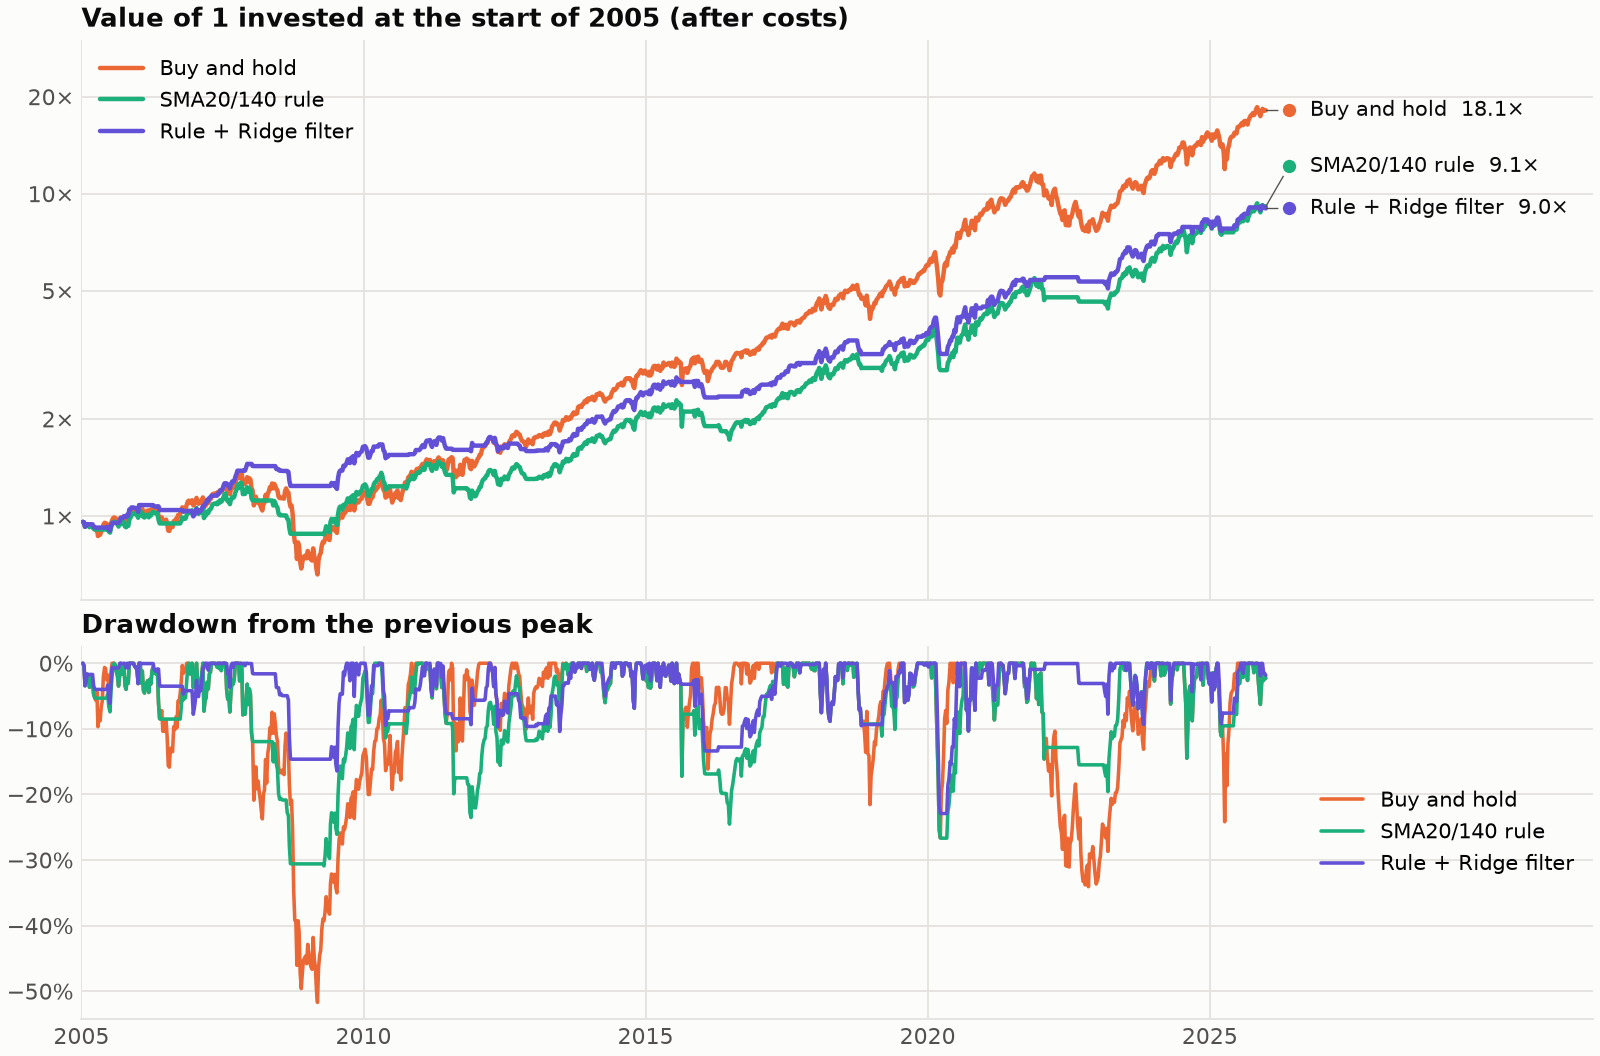
\includegraphics[width=\textwidth]{figures/fig3_qqq_filter.png}
\caption{QQQ: buy-and-hold, the SMA20/140 rule, and the rule with the Ridge filter, 2005--2025. The rule and the filtered rule end at almost the same value; the filtered rule is invested in 51\% of the weeks instead of 79\% and has smaller drawdowns.}
\label{fig:qqq-filter}
\source{\texttt{reports/exhibits/equity\_weekly.csv}}
\end{figure}

Over 2005--2025 the filter keeps 560 of the rule's 864 weeks. Total return is unchanged (11.0\% a year against 11.1\%), exposure falls from 79\% to 51\%, holding CAGR rises from 14.3\% to 22.7\%, and the maximum drawdown falls from 31\% to 23\%. In 2019--2025, the period we held out, holding CAGR rises from 23.2\% to 33.4\%, and total return is 16.1\% against 18.0\%. The filter does not beat buy-and-hold on total return in either period.

Four checks show that the improvement in holding CAGR is not an accident of which weeks happened to be dropped. They use the daily-marked account.

\begin{itemize}
\tightlist
\item
  \textbf{Kept against dropped weeks.} Over 2005--2025 the weeks the filter keeps return +44 basis points on average, and the weeks it drops return +1 basis point (\(t = 2.5\) for the difference). The forecast correlates 0.09 with the realized return over the whole period (\(t = 2.6\)) and 0.14 in 2019--2025.
\item
  \textbf{Year by year.} Kept weeks have a higher average return than dropped weeks in 17 of 21 calendar years (sign test, \(p = 0.004\)).
\item
  \textbf{Placebo.} We shift the filter's keep/drop sequence in time 300 times within the rule's weeks, which preserves how often and how persistently it steps aside. The actual holding CAGR is at the 99th percentile of these placebos in 2005--2018, the 92nd in 2019--2025 and the 99th over the whole period.
\item
  \textbf{Costs.} At 10 basis points per side, holding CAGR is 21.6\% against 14.2\% for the rule; at 20 basis points, 19.2\% against 13.9\%. The filter trades about ten times a year.
\end{itemize}

\subsection{Where the effect comes from}

The redesign changed the features and the target at the same time. Table 7 separates the two, and Table 8 compares models. Both use the rule's weeks and a one-week horizon, and they report the change in holding CAGR relative to the unfiltered rule.

\begin{table}[H]
\centering\small
\caption{Features and target: change in holding CAGR against the unfiltered rule, in percentage points, for 2005--2018 / 2019--2025. Averages over three thresholds (first row) or over five feature sets and three thresholds (second row).}
\label{tab:features-target}
\fittable{tables/tab07_features_target}
\end{table}
\begin{table}[H]
\centering\small
\caption{Models on the market-state features: change in holding CAGR against the unfiltered rule. Each model is run on five feature sets and three thresholds.}
\label{tab:models}
\fittable{tables/tab08_models}
\source{\texttt{results/qqq\_state/QQQ\_sma20\_140/grid.csv}}
\end{table}
\begin{table}[H]
\centering\small
\caption{Fitted Ridge coefficients of the reference configuration. Coefficients are per one standard deviation of the feature, in standard deviations of the weekly return; the next column converts them to basis points. The last fit uses 943 rule weeks from 2000 to 2024 ($\alpha = 10$; intercept 0.090, or 25.6 bp; in-sample $R^2$ 4.4\%).}
\label{tab:coefficients}
\fittable{tables/tab09_coefficients}
\source{\texttt{reports/exhibits/ridge\_coefficients.csv}}
\end{table}

\textbf{Both changes are needed.} With the original price features nothing works, whatever the target. With the new features and the old direction target, there is a gain in 2005--2018 and none in 2019--2025. Only new features together with the return target give a gain in both periods (Table 7). The logistic regression weighted by the size of the return sits between the two targets, which fits the same reading: the more of the return's size the model sees, the better it does.

\textbf{The result belongs to regularized linear regression.} Ridge with either penalty and the Lasso beat the unfiltered rule in 73\% to 100\% of their configurations in both periods (Table 8). The reference configuration, Ridge with \(\alpha = 10\), is the least consistent of the three, so the result does not depend on that particular penalty. Tree models and nearest neighbours do not beat the rule reliably on this sample. We read this as a consequence of the small sample and the weak signal; we have not tested that explanation directly.

\textbf{Which features matter.} With the breadth block alone, holding CAGR is 16.2\% in 2005--2018 and 32.2\% in 2019--2025, close to the 17.7\% and 33.5\% of all 16 features on the same account. The volatility block alone gives 7.7\% and 24.7\%, against 10.1\% and 23.4\% for the unfiltered rule, so it does not carry the result on its own. A Lasso fit keeps a handful of features. It lowers the forecast when all sectors are above their 100-day average, when many members are near 52-week highs, when dispersion is high and when the VIX has been rising. It raises the forecast when long-term breadth is high and when the VIX level is high. In words: step aside when the advance is crowded and extended, and stay when it is broad but nervous.

\textbf{The fitted model.} Table 9 shows the model itself: the coefficients of the last annual fit, estimated on 943 rule weeks from 2000 to 2024. Features are standardized and the target is in standard deviations of the weekly return (2.83\%), so each coefficient is the change in the forecast for a one-standard-deviation change in the feature. A one-standard-deviation rise in realized volatility lowers the forecast by 66 basis points, and in sector breadth by 61. A one-standard-deviation rise in long-term breadth raises it by 41. The intercept is 25.6 basis points, the average return of a rule week, so a week is dropped when the features together subtract more than that. The model explains little of the weekly variation: its in-sample \(R^2\) is 4.4\%.

The coefficients are stable across the 21 annual fits. Nine of the sixteen never change sign, including the four largest, and the coefficient vectors of the first fit (2005) and the last fit (2025) have a correlation of 0.79. The VIX level is the main exception: its coefficient is negative in the five fits up to 2009 and positive from 2010 on.

Realized volatility, the VIX level and implied minus realized variance are closely related, so their coefficients should not be read one at a time. In particular, the negative coefficient on implied minus realized variance does not contradict Bollerslev, Tauchen and Zhou (2009). Taken alone, the highest third of this variable is followed by the highest returns: 43 basis points a week in 2000--2018, against 14 and $-$2 in the other two thirds.

\textbf{The information is short-lived.} With features delayed by one week, holding CAGR in 2005--2018 falls from 17.7\% to 8.2\%, below the unfiltered rule. In 2019--2025 a one-week delay does no harm (34.1\%), and a two-week delay cuts holding CAGR to 15.4\%.

\subsection{The three-component strategy}

The filter alone raises the return per week invested and leaves total return unchanged, because half of the weeks are spent in cash. The momentum ranking addresses exactly this: it replaces the index fund by the ten strongest stocks in the weeks the filter keeps. Table 10 shows all eight combinations of the three components.

\begin{table}[H]
\centering\small
\caption{Ablation with a ten-stock book. The walk-forward columns refit the Ridge model every year; the reverse-time column uses one model fitted on 2009--2025 (Section~7.4). Period columns give CAGR (\%) / holding CAGR (\%) / Sharpe ratio.}
\label{tab:ablation}
\fittable{tables/tab10_ablation}
\source{\texttt{results/ablation/grid.csv}}
\end{table}
\begin{figure}[!htbp]
\centering
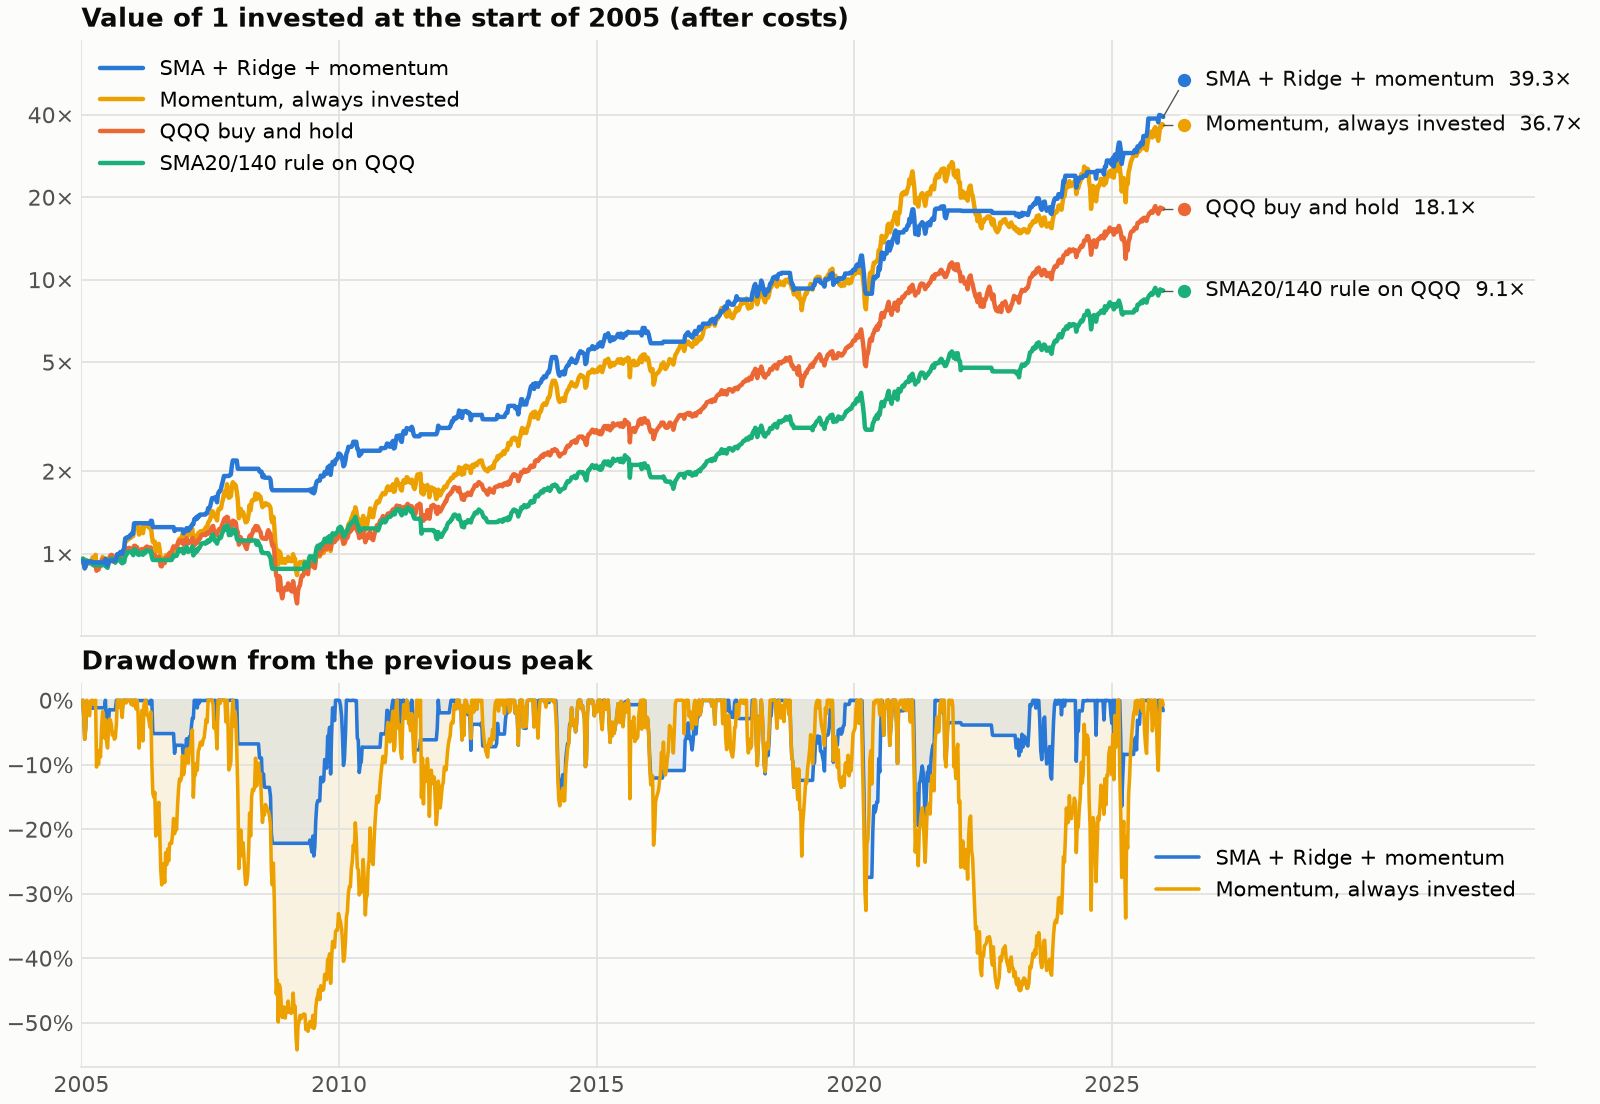
\includegraphics[width=\textwidth]{figures/fig4_three_component.png}
\caption{The three-component strategy against an always-invested momentum portfolio, QQQ buy-and-hold and the SMA rule, 2005--2025. The two momentum portfolios end at a similar value; the three-component strategy gets there while invested in about half of the weeks and with half of the drawdown.}
\label{fig:three-component}
\source{\texttt{reports/exhibits/equity\_weekly.csv}}
\end{figure}

\textbf{The combined strategy.} In 2005--2018 the three-component portfolio has the highest CAGR, holding CAGR and Sharpe ratio of the eight strategies. In 2019--2025 it has the highest holding CAGR. Its CAGR of 23.0\% is within half a point of the always-invested momentum portfolio (23.4\%) and of buy-and-hold (22.6\%), and its Sharpe ratio of 1.04 is level with the three QQQ strategies that reach 1.01 to 1.06. Over 2005--2025 it earns 19.1\% a year with a Sharpe ratio of 1.07, is invested in 51\% of the weeks, and has a maximum drawdown of about 27\%. The always-invested momentum portfolio earns 18.7\% with a Sharpe ratio of 0.76 and a drawdown of 54\%.

\textbf{What each component adds} (2005--2025):

\begin{itemize}
\tightlist
\item
  \textbf{Without the Ridge filter} (SMA + momentum), holding CAGR falls from 40.7\% to 21.8\% and the Sharpe ratio from 1.07 to 0.81.
\item
  \textbf{Without the SMA rule} (Ridge + momentum), the Sharpe ratio falls to 0.85 and the drawdown rises to 37\%. In 2001--2008 this version earns 2.9\% a year against 11.2\%.
\item
  \textbf{Without the momentum ranking} (SMA + Ridge on QQQ), CAGR falls from 19.1\% to 11.0\%.
\end{itemize}

\textbf{Why momentum belongs in the strategy.} The two additions repair each other's weakness. The filter's weakness is low exposure, and momentum raises the return of the weeks that remain. Momentum's weakness is the crash documented by Daniel and Moskowitz (2016), and the trend rule with the filter takes the portfolio out of the market in most of those weeks: the drawdown of the momentum portfolio falls from 54\% to about 27\%.

\begin{table}[H]
\centering\small
\caption{Sensitivity to the number of stocks, annual walk-forward. Period columns give CAGR (\%) / holding CAGR (\%) / Sharpe ratio.}
\label{tab:book-size}
\fittable{tables/tab11_book_size}
\source{\texttt{results/ablation/grid.csv}}
\end{table}

\textbf{The number of stocks.} Table 11 repeats the comparison for 20 and 30 names. In every period and for every book size, the three-component portfolio has a higher holding CAGR and Sharpe ratio than the always-invested momentum portfolio of the same size. The level depends on concentration, however. With 20 or 30 names, total return is below the always-invested portfolio in 2019--2025, and the stock book no longer adds anything to the QQQ version of the strategy in that period (14.9 / 30.7 / 0.84 with 20 names against 16.1 / 33.4 / 1.06 on QQQ). A ten-stock book holds 10\% in each name, so its results also carry more stock-specific risk.

\textbf{The PLTR example again.} Figure 5 adds the three-component portfolio to Figure 2. PLTR was in the momentum top ten throughout. The portfolio bought it at the open on 2 June 2025 at 131.44, when QQQ's trend rule switched on and the Ridge forecast was positive, and held it for ten weeks, a gain of 41.9\%. On Friday 8 August the forecast turned negative, and the portfolio sold at the next open, on 11 August, at 186.47. That is 0.3\% below the highest close PLTR had reached until then. Over the following three weeks, in which the dual-SMA rule on the stock stayed invested, PLTR lost 18.9\%. On 29 August the forecast turned positive again, and the portfolio bought the stock back at the open on 2 September at 151.20.

The signal is about the market, not about PLTR. The forecast is for QQQ's return in the following week, and the portfolio sold all ten of its stocks on 11 August. Over the whole of 2025 the portfolio was invested in 27 of 52 weeks; PLTR returned 110\% over those weeks and 6\% over the other 25.

One episode is an illustration. The filter is wrong often: in February and March 2020 it stayed invested in three of the four weeks of the crash, and in June and July 2016 it stayed out for six weeks while QQQ rose 12.8\%. The evidence is the average over all weeks in Tables 6 and 10 and the tests of Section 7.1.

\begin{figure}[!htbp]
\centering
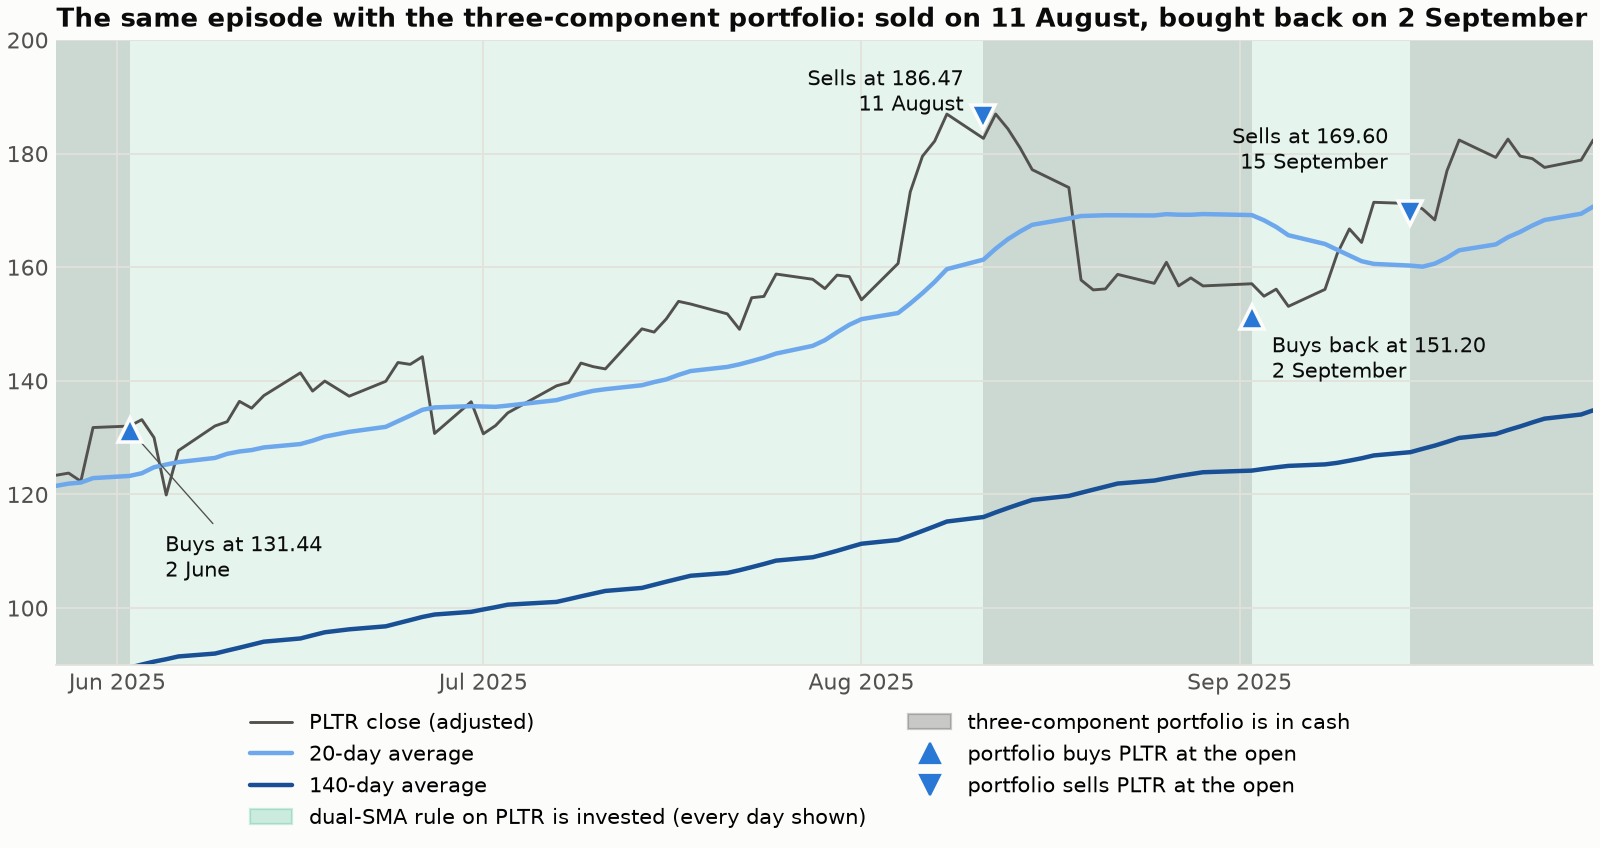
\includegraphics[width=0.95\textwidth]{figures/fig5_example_filter.png}
\caption{The PLTR episode with the three-component portfolio. Grey bands are weeks in which the portfolio is in cash; triangles mark its purchases and sales of PLTR at the weekly open.}
\label{fig:example-filter}
\source{\texttt{reports/exhibits/example\_daily.csv}, \texttt{example\_weeks.csv}}
\end{figure}
\begin{table}[H]
\centering\small
\caption*{\textbf{The PLTR example in numbers.}}
\fittable{tables/tab_example}
\end{table}

\subsection{Robustness}

\textbf{(a) Other moving-average pairs.} The pair 20/140 is one choice among many. We rebuild the whole strategy (the rule's weeks, the Ridge fit, the stock candidates) for 222 pairs with a short window of 1 to 51 days and a long window of 30 to 230 days, and compare each strategy with the plain SMA rule on the same pair.

\begin{table}[H]
\centering\small
\caption{222 moving-average pairs: share of pairs in which the strategy beats the plain SMA rule on the same pair, and the median gain.}
\label{tab:sma-pairs}
\fittable{tables/tab12_sma_pairs}
\source{\texttt{results/ablation/sma\_grid/summary.csv}}
\end{table}
\begin{figure}[p]
\centering
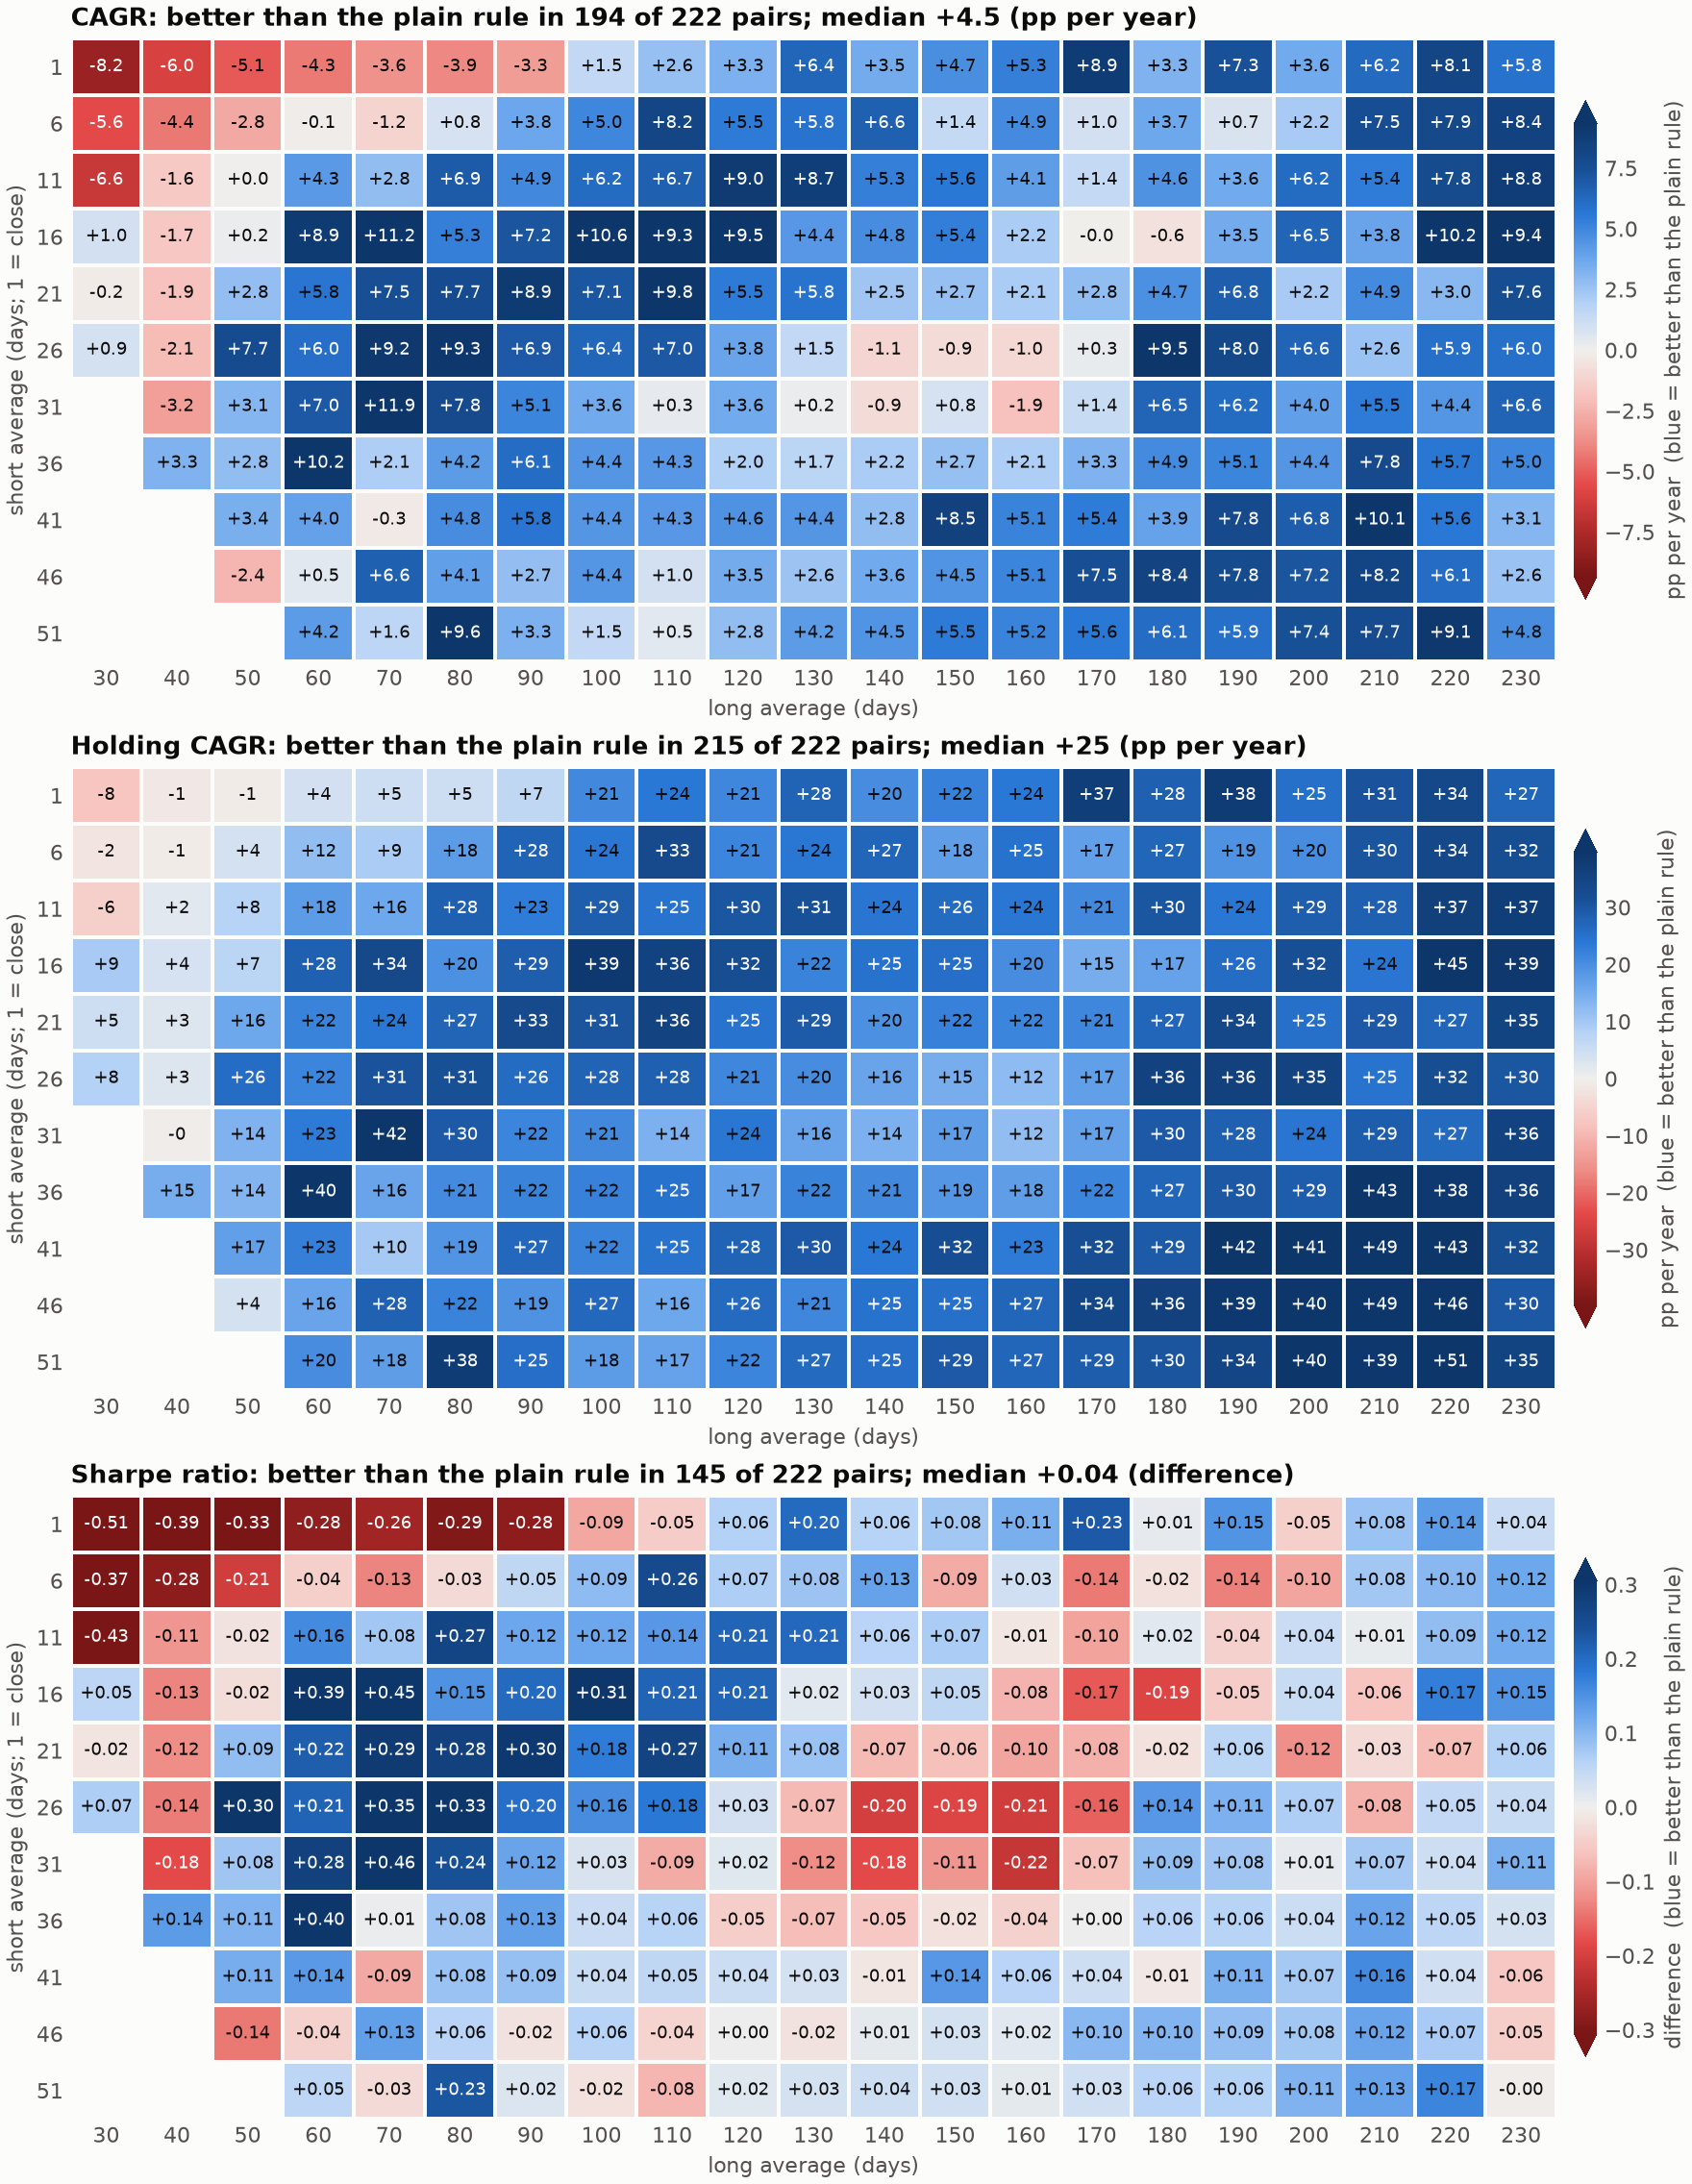
\includegraphics[height=0.84\textheight]{figures/fig6_sma_pairs_2019_2025.png}
\caption{2019--2025, annual walk-forward: gain of the three-component strategy (top ten) over the plain SMA rule on the same pair, for each of 222 pairs. Each cell is one pair; blue means the strategy is better.}
\label{fig:sma-pairs}
\source{\texttt{results/ablation/sma\_grid/gain\_vs\_sma.csv}}
\end{figure}

With ten stocks, the strategy has a higher holding CAGR than the plain rule in 97\% to 100\% of the pairs in every period (Table 12). Total return is higher in 96\% of the pairs in 2005--2018 and in 87\% in 2019--2025; the Sharpe ratio is higher in 97\% and 65\%. Most of the pairs in which total return is lower in 2019--2025 have a long average of 60 days or less; among the pairs with a long average of 70 days or more, the strategy is ahead in 94\% (Figure 6). The second block of Table 12 repeats the point of Section 7.3: the filter on QQQ alone raises holding CAGR in 91\% to 100\% of the pairs, and it raises total return in only 16\% to 32\% of them in the walk-forward periods.

\textbf{(b) A test that runs backwards in time.} The walk-forward cannot score the years before 2005, which include the end of the dot-com decline. We therefore fit one model on 2009--2025, freeze it, and apply it to 2001--2008. QQQ lost 8.1\% a year in that period. The 2001--2008 column of Table 10 gives the result: the SMA rule earns $-$0.5\% a year, the rule with the filter 2.3\%, and the three-component portfolio 11.2\% with a drawdown of 31\%. Across the 222 pairs the three-component portfolio beats the plain rule on all three measures in every pair (Table 12). This test uses future data to fit the model, so it shows that the relation is stable across time; it is not a history that could have been traded. It is also sensitive to a few weeks. Fitting on 2008--2025 instead adds only 14 training weeks from early 2008, and the filter changes noticeably: on 2001--2007 it keeps 62\% of the rule's weeks instead of 77\%, and its holding CAGR there is 27.8\% against 6.6\% for the rule.

\textbf{(c) Leave one period out.} We cut 2001--2025 into four periods and score each with a Ridge model fitted on the other three (plus 2000) and then frozen. Training weeks within 14 days of the test period are dropped. For 2019--2025 the model uses past data only; for the three earlier periods it also uses later years, so those are cross-validation results. The last column chains the four sets of forecasts into one account.

\begin{table}[H]
\centering\small
\caption{Leave-one-period-out test at SMA20/140 with a ten-stock book. Each period is scored by a model fitted on the other three. Period columns give CAGR (\%) / holding CAGR (\%) / Sharpe ratio.}
\label{tab:blocks}
\fittable{tables/tab13_blocks}
\source{\texttt{results/ablation/blocks/}}
\end{table}
\begin{table}[H]
\centering\small
\caption{Leave-one-period-out test over 222 moving-average pairs: the three-component strategy (top ten) against the plain SMA rule on the same pair.}
\label{tab:blocks-pairs}
\fittable{tables/tab14_blocks_pairs}
\end{table}
\begin{table}[H]
\centering\small
\caption{Leave-one-period-out test: share of the 222 pairs in which the three-component strategy (top ten) is better than each other combination.}
\label{tab:blocks-versus}
\fittable{tables/tab15_blocks_versus}
\end{table}
\begin{sidewaysfigure}[p]
\centering
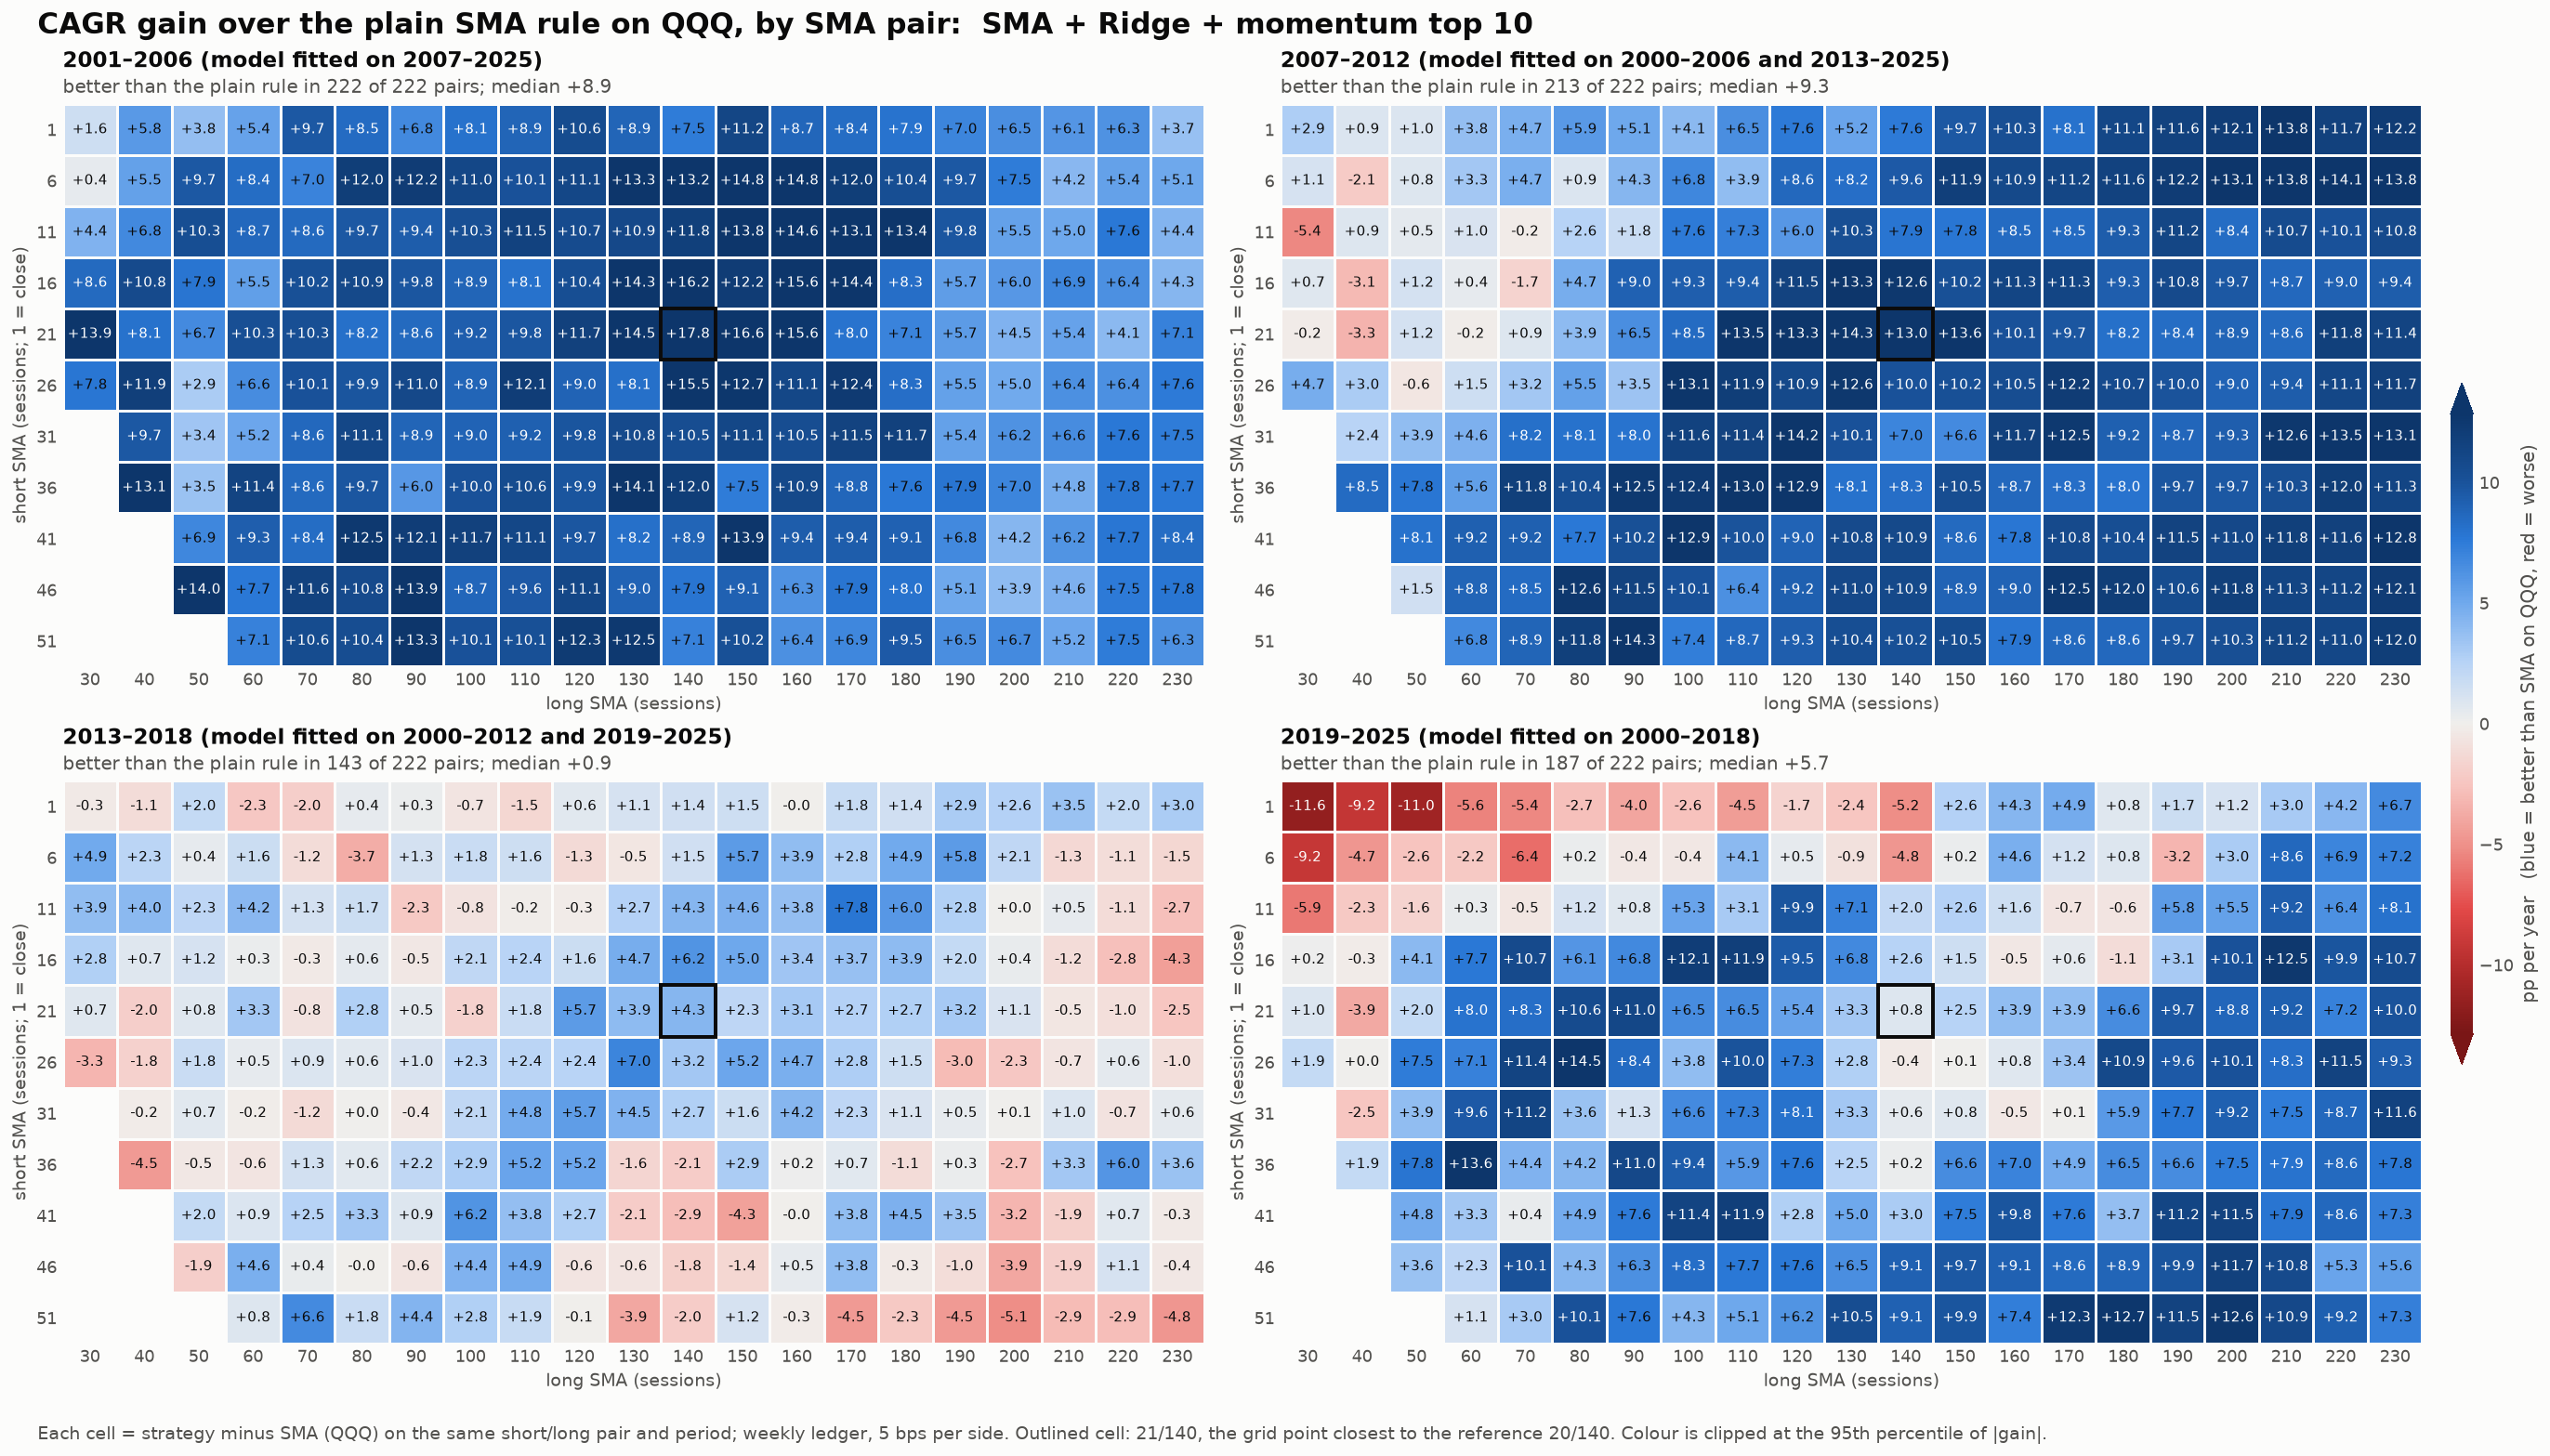
\includegraphics[width=\textheight,height=0.88\textwidth,keepaspectratio]{figures/fig7_blocks_cagr.png}
\caption{Leave-one-period-out test: CAGR gain of the three-component strategy (top ten) over the plain SMA rule on the same pair, one panel per test period.}
\label{fig:blocks-cagr}
\source{\texttt{results/ablation/blocks/}}
\end{sidewaysfigure}

Over the chained period 2001--2025 the three-component portfolio has the highest Sharpe ratio of the eight strategies (1.05; the next is 0.86) and the highest holding CAGR, and its total return of 18.6\% a year is level with the best (18.7\%). The four periods differ.

\begin{itemize}
\tightlist
\item
  \textbf{2001--2006 and 2007--2012}, the two periods with bear markets: the strategy beats the plain rule in 96\% to 100\% of the pairs on every measure.
\item
  \textbf{2013--2018}, a calm rising market: holding CAGR is higher in almost every pair, and total return and the Sharpe ratio are higher in 64\% of them. At 20/140 the Sharpe ratio is still the highest of the eight, and total return is 19.5\% a year against 25.1\% for the always-invested momentum portfolio. The filter costs return in this period: Table 15 shows the three-component portfolio below the momentum portfolios on total return in nearly every pair.
\item
  \textbf{2019--2025}: holding CAGR is higher in 96\% of the pairs, total return in 84\% and the Sharpe ratio in 66\%. With the model frozen at the end of 2018, CAGR at 20/140 is 20.7\%. The annual walk-forward of Table 10, which refits every year, gives 23.0\%.
\end{itemize}

Table 15 adds a qualification about the SMA rule. Over the chained period, the version without it (Ridge + momentum) has a higher total return than the three-component portfolio for most pairs; the three-component portfolio is ahead on holding CAGR in 80\% of the pairs and on the Sharpe ratio in 70\%. In this test the SMA rule contributes to risk control, not to total return.

In short, the leave-one-period-out test supports the result for the whole period and for holding CAGR in every period. It also shows that the gain in total return comes from the periods that contain bear markets.

\subsection{What does not hold}

\begin{itemize}
\tightlist
\item
  \textbf{Total return in rising markets.} In 2019--2025 the strategy's total return is about equal to an always-invested momentum portfolio and to buy-and-hold in the walk-forward (23.0\% against 23.4\% and 22.6\%), and lower with a model frozen in 2018 (20.7\%). In 2013--2018 it is clearly lower than the momentum portfolio. On QQQ alone, the filter does not raise total return above buy-and-hold in either walk-forward period.
\item
  \textbf{Sharpe ratio in 2019--2025.} It is level with the QQQ strategies (1.04 against 1.01 to 1.06), not above them.
\item
  \textbf{Concentration.} With 20 or 30 stocks the gain over the QQQ version disappears in 2019--2025 (Table 11).
\item
  \textbf{Model type.} Only regularized linear regressions work. Trees and nearest neighbours do not (Table 8).
\item
  \textbf{Statistical strength.} The \(t\)-statistics are about 2.5, below the threshold of 3 that Harvey, Liu and Zhu (2016) recommend for newly proposed factors.
\item
  \textbf{Dependence on a few weeks.} The reverse-time result changes a lot when 14 crash weeks are added to the training set (Section 7.4).
\item
  \textbf{Other markets.} All tests use the Nasdaq-100. Limited checks on other index funds were mixed, and we do not claim that the result carries over.
\end{itemize}

\section{Discussion and limitations}

\textbf{Why would a filter of this kind work?} The Lasso reading in Section 7.2 has a simple interpretation. Inside an uptrend, the weeks to avoid are those in which the advance is crowded (all sectors up, many stocks at their highs) and the stocks have started to move apart. The weeks to keep are those in which long-term breadth is intact and investors are nervous, as shown by a high VIX. This is in line with two findings: stock returns are higher after implied variance has been high relative to realized variance (Bollerslev, Tauchen and Zhou, 2009), and the return to providing liquidity rises with the VIX (Nagel, 2012). It is the opposite of what a volatility filter or a direction classifier does. It also explains our first negative result: the first design was built to learn the wrong lesson from the right data.

\textbf{What the strategy is.} The three-component portfolio is best described as a risk-managed momentum strategy. Over a period that includes bear markets it earns about the return of a momentum portfolio with half the time in the market and half the drawdown. In a long rising market it earns less than staying invested.

\textbf{Limitations.}

\begin{itemize}
\tightlist
\item
  \textbf{Status of the evidence.} The first design was specified in our proposal before any result was seen, and its negative result stands. The redesign came afterwards and is exploratory. Its cleanest test is 2019--2025.
\item
  \textbf{One signal, one market.} All strategies share the same timing signal and the same stock universe, so the rows of the ablation tables are not independent pieces of evidence.
\item
  \textbf{Sample size.} There are 864 rule weeks in 2005--2025, and a small number of crash weeks carry much of the information.
\item
  \textbf{Data.} The constituent data are a vendor candidate package with open quality flags, and prices are adjusted closes used as a total-return approximation.
\item
  \textbf{Costs and execution.} We charge 5 basis points per side and assume fills at the open. The ten-stock book turns over about 14 times a year, so higher costs would matter more for it than for the QQQ version.
\item
  \textbf{Holding CAGR.} It measures selection, and it is inflated when exposure is low. We report it with exposure for that reason.
\end{itemize}

\section{Conclusion}

A classifier that predicts the direction of next week's return from price features adds nothing to a moving-average rule, for reasons we could identify in the data: the sign of the return varies little across market states, the features repeat what the rule already knows, and what such a model can learn is to avoid volatility, which is the wrong action inside an uptrend. A Ridge regression on market-state features that forecasts the size of the return does add something. It lets the rule earn the same total return in half the time, and combined with a ten-stock momentum portfolio it produces a strategy with a higher Sharpe ratio and a much smaller drawdown than any of its parts over 2005--2025. The advantage comes from periods with bear markets. In rising markets the strategy keeps pace with an always-invested portfolio at best. The method that worked was the simplest one taught in the course, applied to the right target and the right information.

\section*{References}
\addcontentsline{toc}{section}{References}

\begin{reflist}
\item
  Bailey, D. H., Borwein, J. M., López de Prado, M., \& Zhu, Q. J. (2014). Pseudo-mathematics and financial charlatanism: The effects of backtest overfitting on out-of-sample performance. \emph{Notices of the American Mathematical Society}, 61(5), 458--471.
\item
  Bollerslev, T., Tauchen, G., \& Zhou, H. (2009). Expected stock returns and variance risk premia. \emph{Review of Financial Studies}, 22(11), 4463--4492.
\item
  Brock, W., Lakonishok, J., \& LeBaron, B. (1992). Simple technical trading rules and the stochastic properties of stock returns. \emph{Journal of Finance}, 47(5), 1731--1764.
\item
  Cederburg, S., O'Doherty, M. S., Wang, F., \& Yan, X. (2020). On the performance of volatility-managed portfolios. \emph{Journal of Financial Economics}, 138(1), 95--117.
\item
  Christoffersen, P. F., \& Diebold, F. X. (2006). Financial asset returns, direction-of-change forecasting, and volatility dynamics. \emph{Management Science}, 52(8), 1273--1287.
\item
  Daniel, K., \& Moskowitz, T. J. (2016). Momentum crashes. \emph{Journal of Financial Economics}, 122(2), 221--247.
\item
  Faber, M. T. (2007). A quantitative approach to tactical asset allocation. \emph{The Journal of Wealth Management}, 9(4), 69--79.
\item
  Gu, S., Kelly, B., \& Xiu, D. (2020). Empirical asset pricing via machine learning. \emph{Review of Financial Studies}, 33(5), 2223--2273.
\item
  Harvey, C. R., Liu, Y., \& Zhu, H. (2016). \ldots{} and the cross-section of expected returns. \emph{Review of Financial Studies}, 29(1), 5--68.
\item
  Hoerl, A. E., \& Kennard, R. W. (1970). Ridge regression: Biased estimation for nonorthogonal problems. \emph{Technometrics}, 12(1), 55--67.
\item
  Israel, R., Kelly, B., \& Moskowitz, T. (2020). Can machines ``learn'' finance? \emph{Journal of Investment Management}, 18(2), 23--36.
\item
  Jegadeesh, N., \& Titman, S. (1993). Returns to buying winners and selling losers: Implications for stock market efficiency. \emph{Journal of Finance}, 48(1), 65--91.
\item
  Joubert, J. F. (2022). Meta-labeling: Theory and framework. \emph{Journal of Financial Data Science}, 4(3), 31--44.
\item
  López de Prado, M. (2018). \emph{Advances in Financial Machine Learning}. Wiley.
\item
  Moreira, A., \& Muir, T. (2017). Volatility-managed portfolios. \emph{Journal of Finance}, 72(4), 1611--1644.
\item
  Moskowitz, T. J., Ooi, Y. H., \& Pedersen, L. H. (2012). Time series momentum. \emph{Journal of Financial Economics}, 104(2), 228--250.
\item
  Nagel, S. (2012). Evaporating liquidity. \emph{Review of Financial Studies}, 25(7), 2005--2039.
\item
  Neely, C. J., Rapach, D. E., Tu, J., \& Zhou, G. (2014). Forecasting the equity risk premium: The role of technical indicators. \emph{Management Science}, 60(7), 1772--1791.
\item
  Sullivan, R., Timmermann, A., \& White, H. (1999). Data-snooping, technical trading rule performance, and the bootstrap. \emph{Journal of Finance}, 54(5), 1647--1691.
\item
  Welch, I., \& Goyal, A. (2008). A comprehensive look at the empirical performance of equity premium prediction. \emph{Review of Financial Studies}, 21(4), 1455--1508.
\item
  Yu, S., Webb, G., \& Lin, B. (2025). The use of index-specific market breadth and index-over-moving-average indicators in stock trading strategies. \emph{Journal of Investing}, 34(2), 83--101.
\item
  Zaremba, A., Szyszka, A., Karathanasopoulos, A., \& Mikutowski, M. (2021). Herding for profits: Market breadth and the cross-section of global equity returns. \emph{Economic Modelling}, 97, 348--364.
\end{reflist}

\appendix
\setcounter{figure}{0}
\renewcommand{\thefigure}{A\arabic{figure}}

\section{Other attempts on the first design}

All of these keep the idea of the first design, a classifier trained on win/lose labels with price-based features. None produced a filter with skill.

\begin{itemize}
\tightlist
\item
  \textbf{The five cases of the proposal} (QQQ with SMA20/60, SMA10/30, SMA40/120 and a 60-day momentum rule; SPY with SMA20/60), test 2019--2025: AUC between 0.46 and 0.55, Brier skill between $-$0.5\% and +0.4\%.
\item
  \textbf{A longer history.} A walk-forward over 2005--2025 and a blocked cross-validation over 2000--2025 give the same answer. For SMA20/60 the rule's holding CAGR is 8.4\% against 14.8\% for buy-and-hold, with a maximum drawdown of 36\% against 53\%.
\item
  \textbf{No SMA rule.} A classifier that times QQQ alone earns about the same as buy-and-hold scaled to the same exposure.
\item
  \textbf{Whole trades instead of weeks.} With trade-level labels on individual stocks (four label definitions), AUC is between 0.46 and 0.54, and over 2005--2025 the models tend to drop the trades with the highest returns.
\item
  \textbf{A weaker base rule.} Across 215 moving-average pairs, a weaker rule makes the classifier less harmful and never useful.
\item
  \textbf{Buying what the classifier rejects.} The result is not stable across periods.
\item
  \textbf{Ranking stocks with the same labels.} Holding the top 20 Nasdaq-100 members by classifier score is not distinguishable from a random choice of 20: the best rules reach the 91st to 97th percentile of a random placebo, with \(t \le 1.6\) on the weekly spread, and weekly re-ranking turns the portfolio over 35 to 60 times a year.
\end{itemize}

\section{Hyperparameters}

\begin{table}[H]
\centering\small
\caption*{\textbf{Settings.}}
\begin{tabularx}{\textwidth}{@{}p{0.24\textwidth}X@{}}
\toprule
Component & Setting \\
\midrule
Ridge filter & $\alpha = 10$; features standardized; missing values set to the training median; target divided by its training standard deviation \\
\addlinespace
Training set & Weeks in which QQQ's SMA20 is above its SMA140, from 2000; refitted every January on all earlier weeks with complete returns \\
\addlinespace
Decision & Hold if the forecast of next week's return is positive \\
\addlinespace
Momentum book & Members with their own SMA20 above SMA140; ranked by 252-day return; top 10 at 10\% each; re-ranked every 4 weeks; a name that leaves the candidate set is sold \\
\addlinespace
Costs & 5 basis points per side on every change in weight \\
\addlinespace
Models compared in Table~\ref{tab:models} & Ridge ($\alpha = 10, 100$), Lasso ($\alpha = 0.02$), gradient boosting (50 trees of depth 1; 100 trees of depth 2), random forest (300 trees, depth 3), 25 nearest neighbours, support vector regression, logistic regression ($C = 0.1$), all on standardized features \\
\bottomrule
\end{tabularx}
\end{table}

\section{Reproducing the results}

All data are in the project repository under \texttt{data/}. From the repository root:

{\scriptsize
\begin{verbatim}
python scripts/run_experiments.py                            # first design, the proposal's five cases
ML_CASE=QQQ:sma20_140 python scripts/run_experiments.py      # first design on SMA20/140 (Table 2)
python scripts/run_robustness.py                             # walk-forward and blocked CV, five cases
ML_CASE=QQQ:sma20_140 python scripts/run_robustness.py       # the same on SMA20/140 (Table 2)
python scripts/run_ml_only.py                                # Appendix A: no SMA rule
python scripts/run_stocks.py --sma 20_140                    # Appendix A: stocks; also 20_60, 10_30, 40_120
python scripts/run_meta_label.py                             # Appendix A: whole trades, rejected trades
python scripts/run_meta_grid.py                              # Appendix A: 215 moving-average pairs
python scripts/prescreen_dev.py > results/prescreen_dev.txt  # pre-screen on data through 2018 (Table 3)
python scripts/run_qqq_state.py                              # Ridge filter and its grid (Tables 7 and 8)
python scripts/diagnose_qqq_state.py                         # kept and dropped weeks, placebo, costs, blocks
python scripts/run_qqq_reverse.py                            # reverse-time test
python scripts/run_stock_rank.py                             # machine-learning stock rankings (Section 6.4)
python scripts/run_ablation.py                               # ablation (Tables 6, 10 and 11)
python scripts/run_ablation_sma_grid.py                      # 222 pairs (Table 12, Figures 6 and A3)
python scripts/run_ablation_blocks.py                        # leave one period out (Tables 13-15, Figure 7)
python scripts/make_report_exhibits.py                       # series behind Figures 1 to 5, Table 9
python scripts/make_report_figures.py                        # Figures 1 to 6
python scripts/make_report_tables.py                         # LaTeX tables; copies Figures 7 and A1 to A3
\end{verbatim}
}

\section{Relation to the proposal}

\begin{table}[H]
\centering\small
\caption*{\textbf{The proposal and this report.}}
\begin{tabularx}{\textwidth}{@{}p{0.14\textwidth}XX@{}}
\toprule
Item & Proposal & This report \\
\midrule
Base rule & SMA20/60 as the main case, four other cases & SMA20/140 throughout; the proposal's cases are in Appendix~A \\
\addlinespace
Filter & Direction classifier on seven price features & Section~5 (no skill), then the redesign of Section~6 \\
\addlinespace
Main metric & CAGR & CAGR with holding CAGR and exposure, added after the first results \\
\addlinespace
Stocks & Not in the main study & Momentum ranking of Nasdaq-100 members, added after the QQQ results \\
\addlinespace
Evaluation & Train 2000--2013, validation 2014--2018, test 2019--2025 & Kept for the first design; the redesign uses an annual walk-forward with 2019--2025 held out, plus the tests of Section~7.4 \\
\bottomrule
\end{tabularx}
\end{table}

\section{Additional figures}

\begin{sidewaysfigure}[p]
\centering
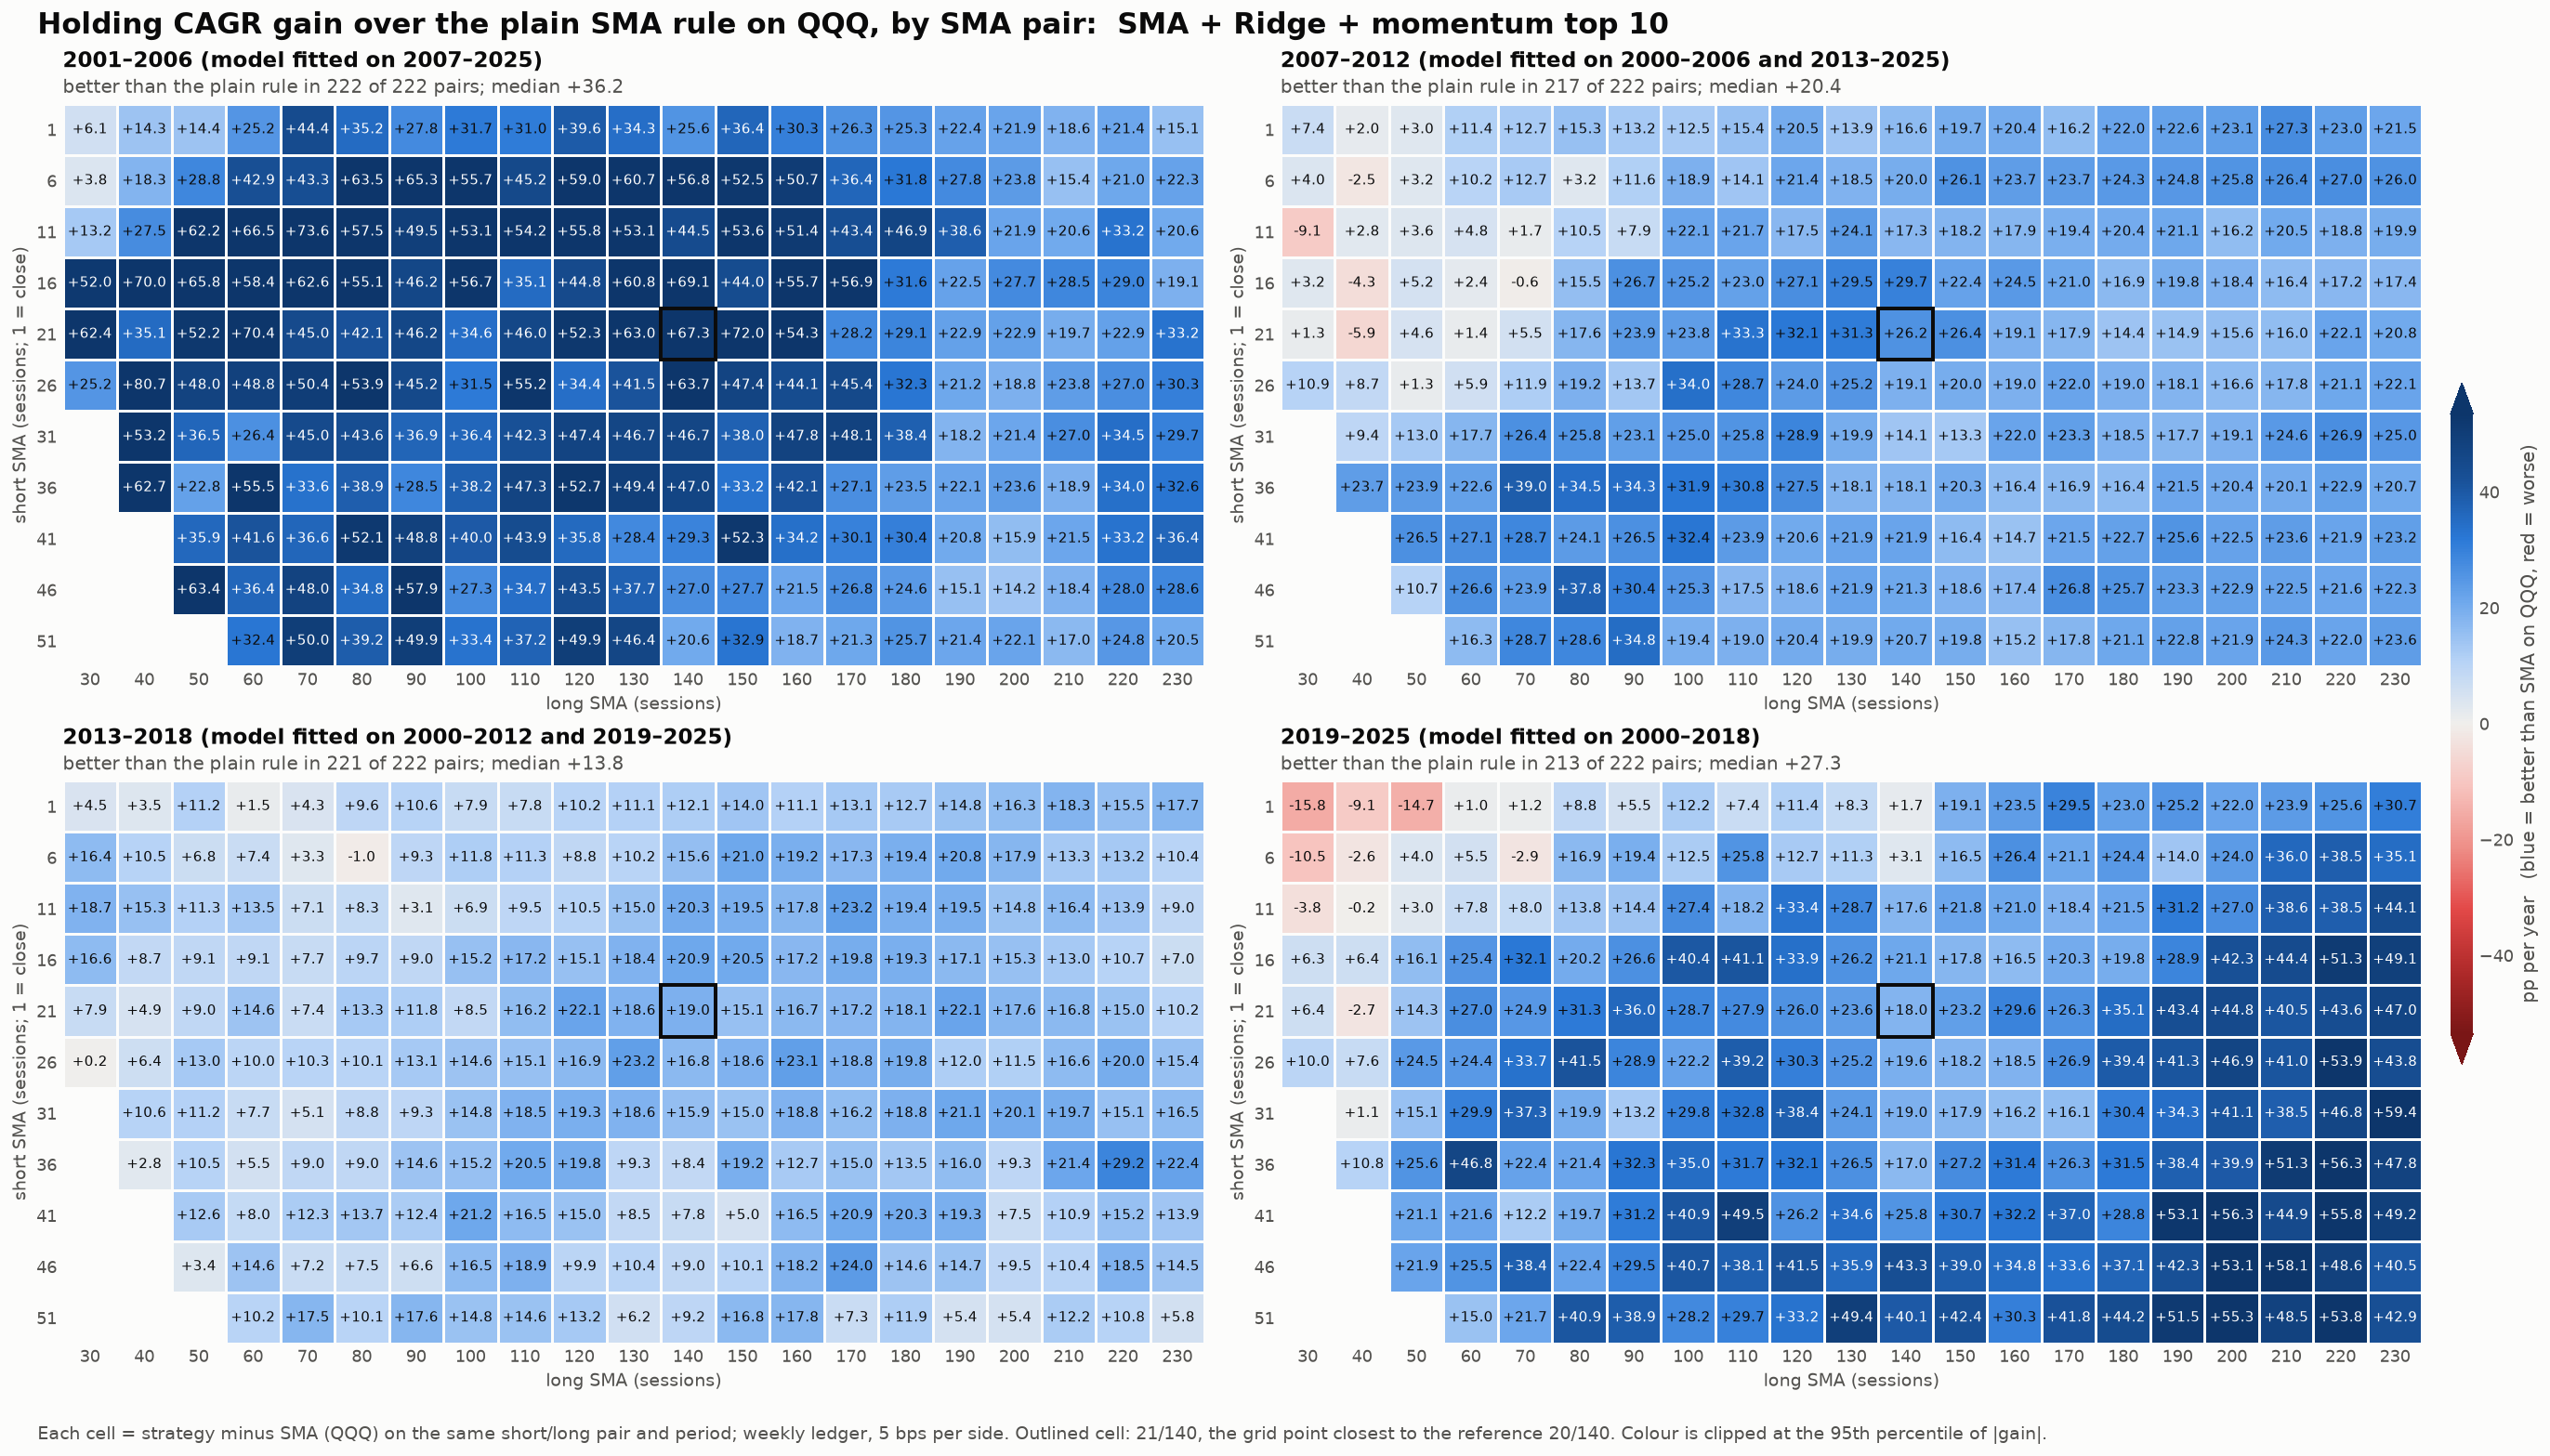
\includegraphics[width=\textheight,height=0.88\textwidth,keepaspectratio]{figures/figA1_blocks_hold_cagr.png}
\caption{Leave-one-period-out test: holding CAGR gain of the three-component strategy (top ten) over the plain SMA rule.}
\label{fig:a1}
\source{\texttt{results/ablation/blocks/}}
\end{sidewaysfigure}
\begin{sidewaysfigure}[p]
\centering
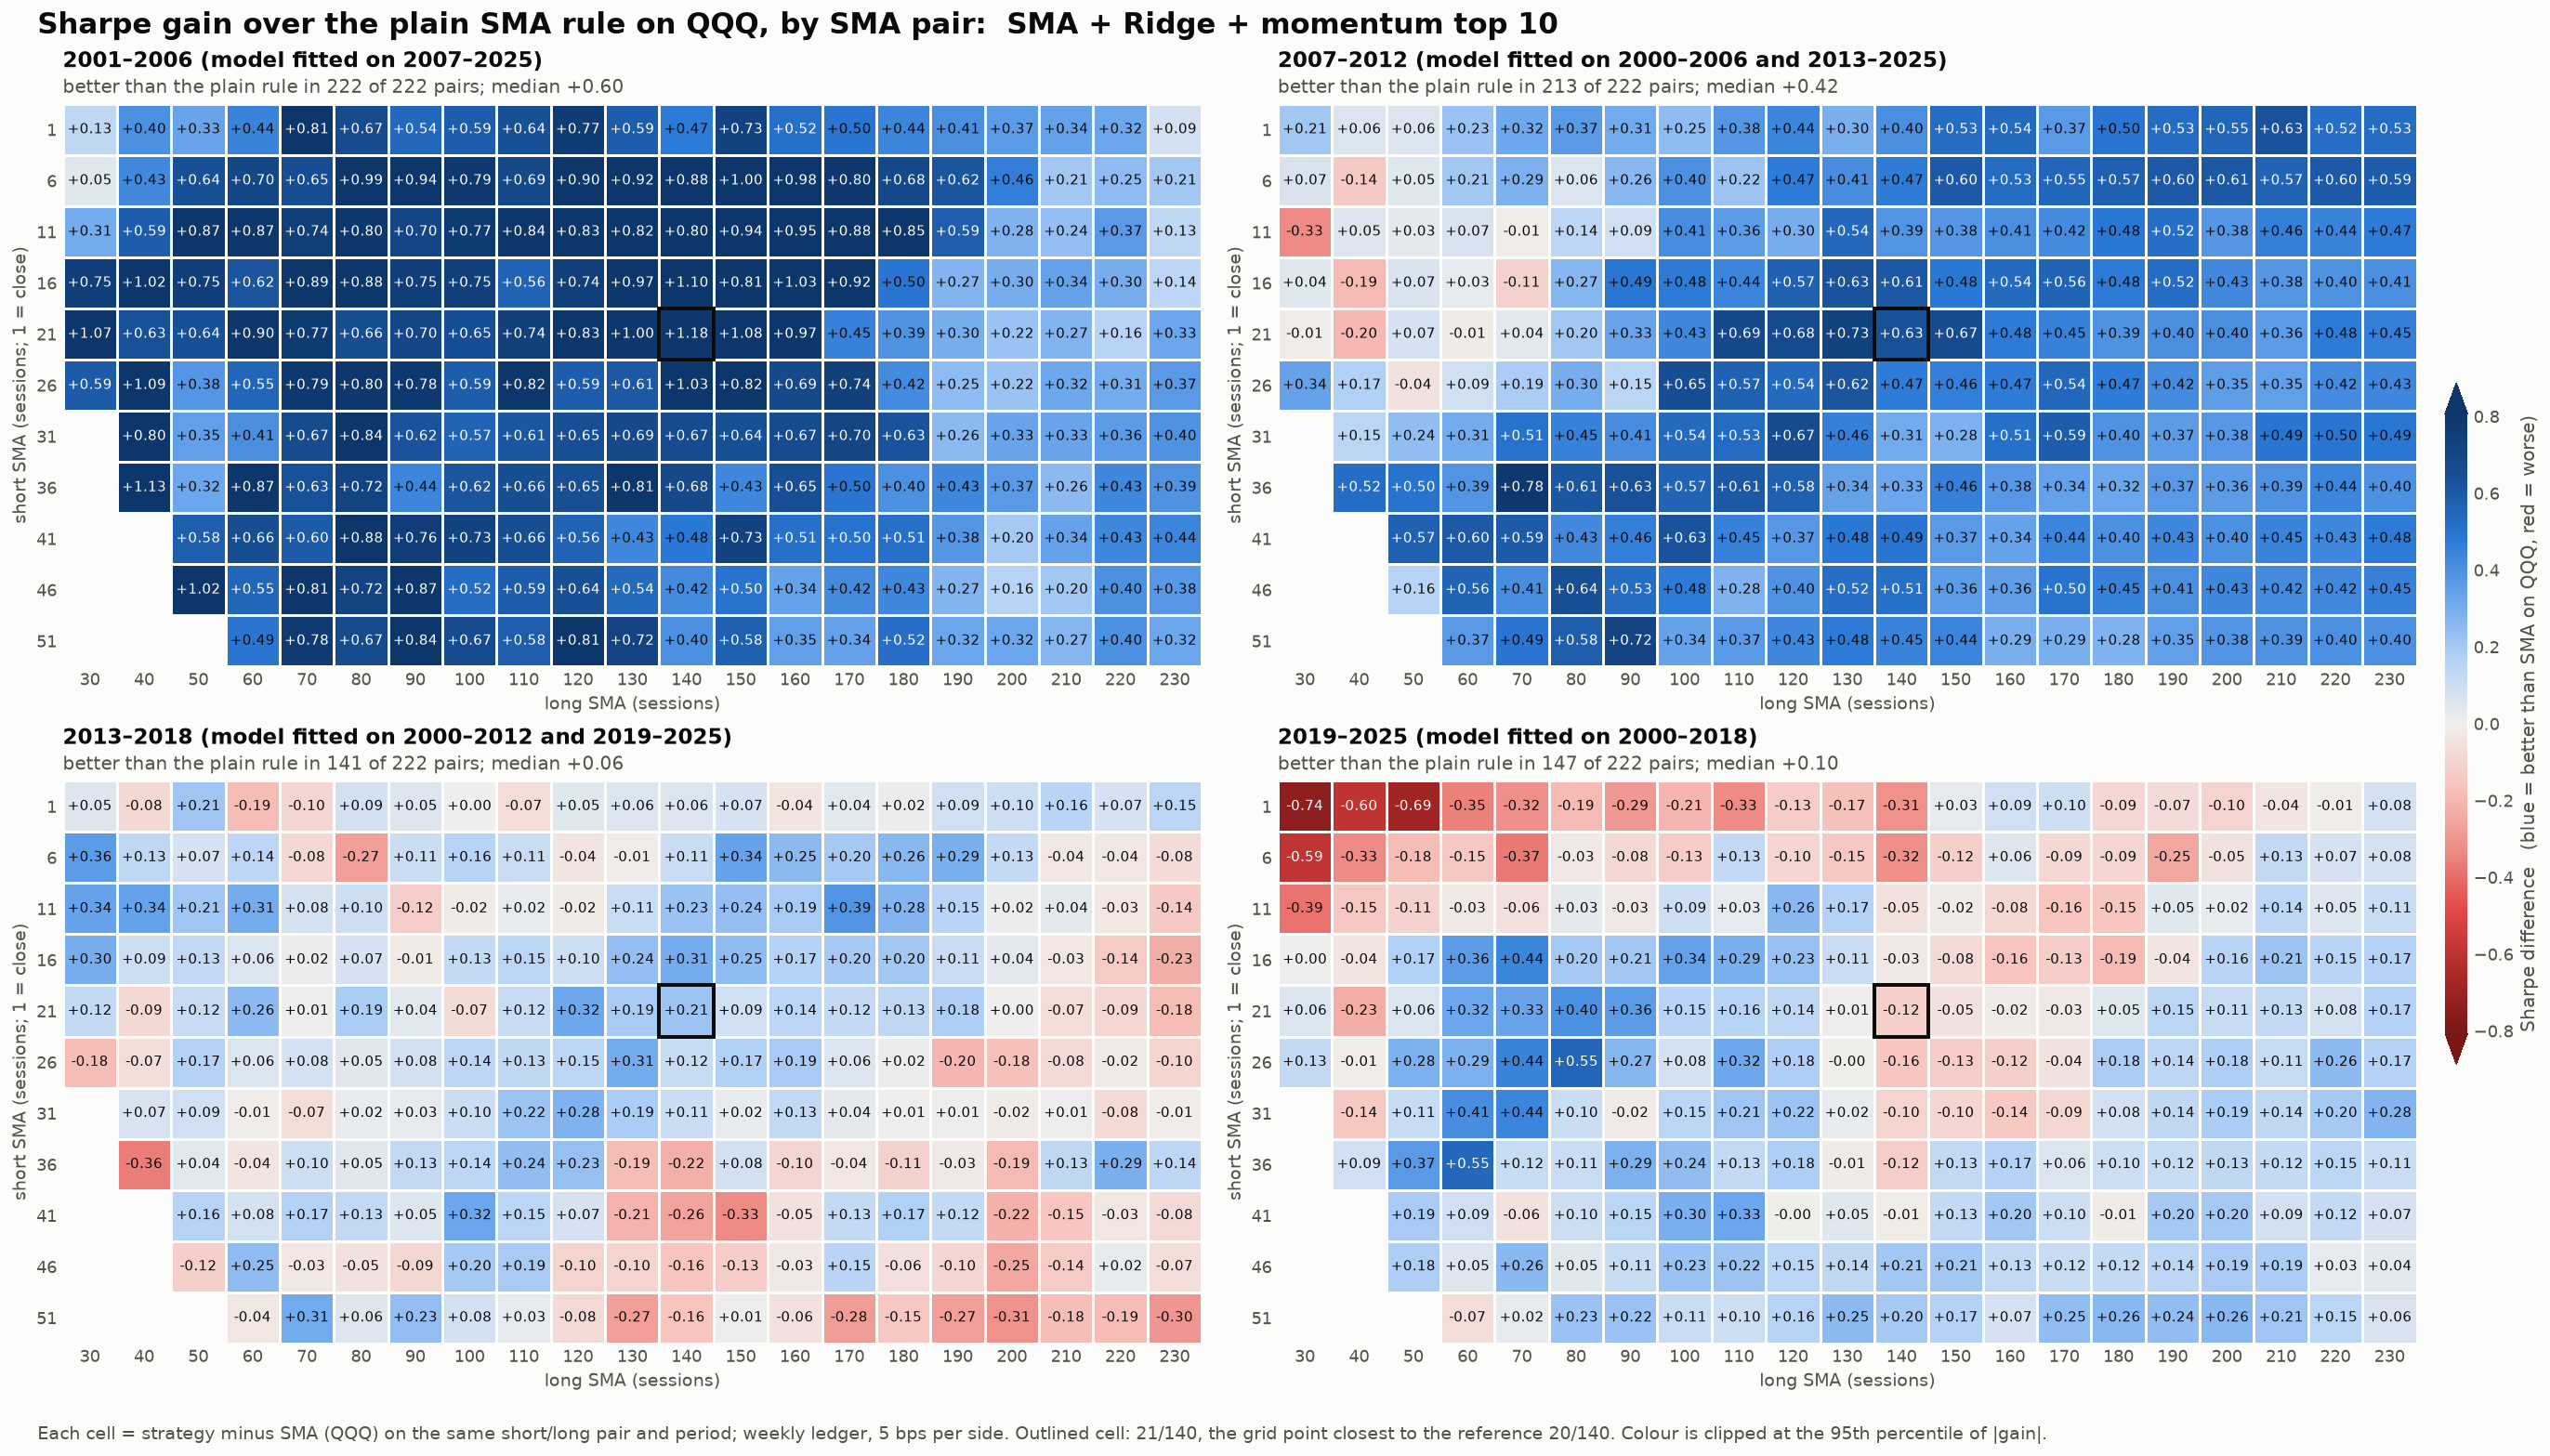
\includegraphics[width=\textheight,height=0.88\textwidth,keepaspectratio]{figures/figA2_blocks_sharpe.png}
\caption{Leave-one-period-out test: Sharpe ratio gain of the three-component strategy (top ten) over the plain SMA rule.}
\label{fig:a2}
\source{\texttt{results/ablation/blocks/}}
\end{sidewaysfigure}
\begin{sidewaysfigure}[p]
\centering
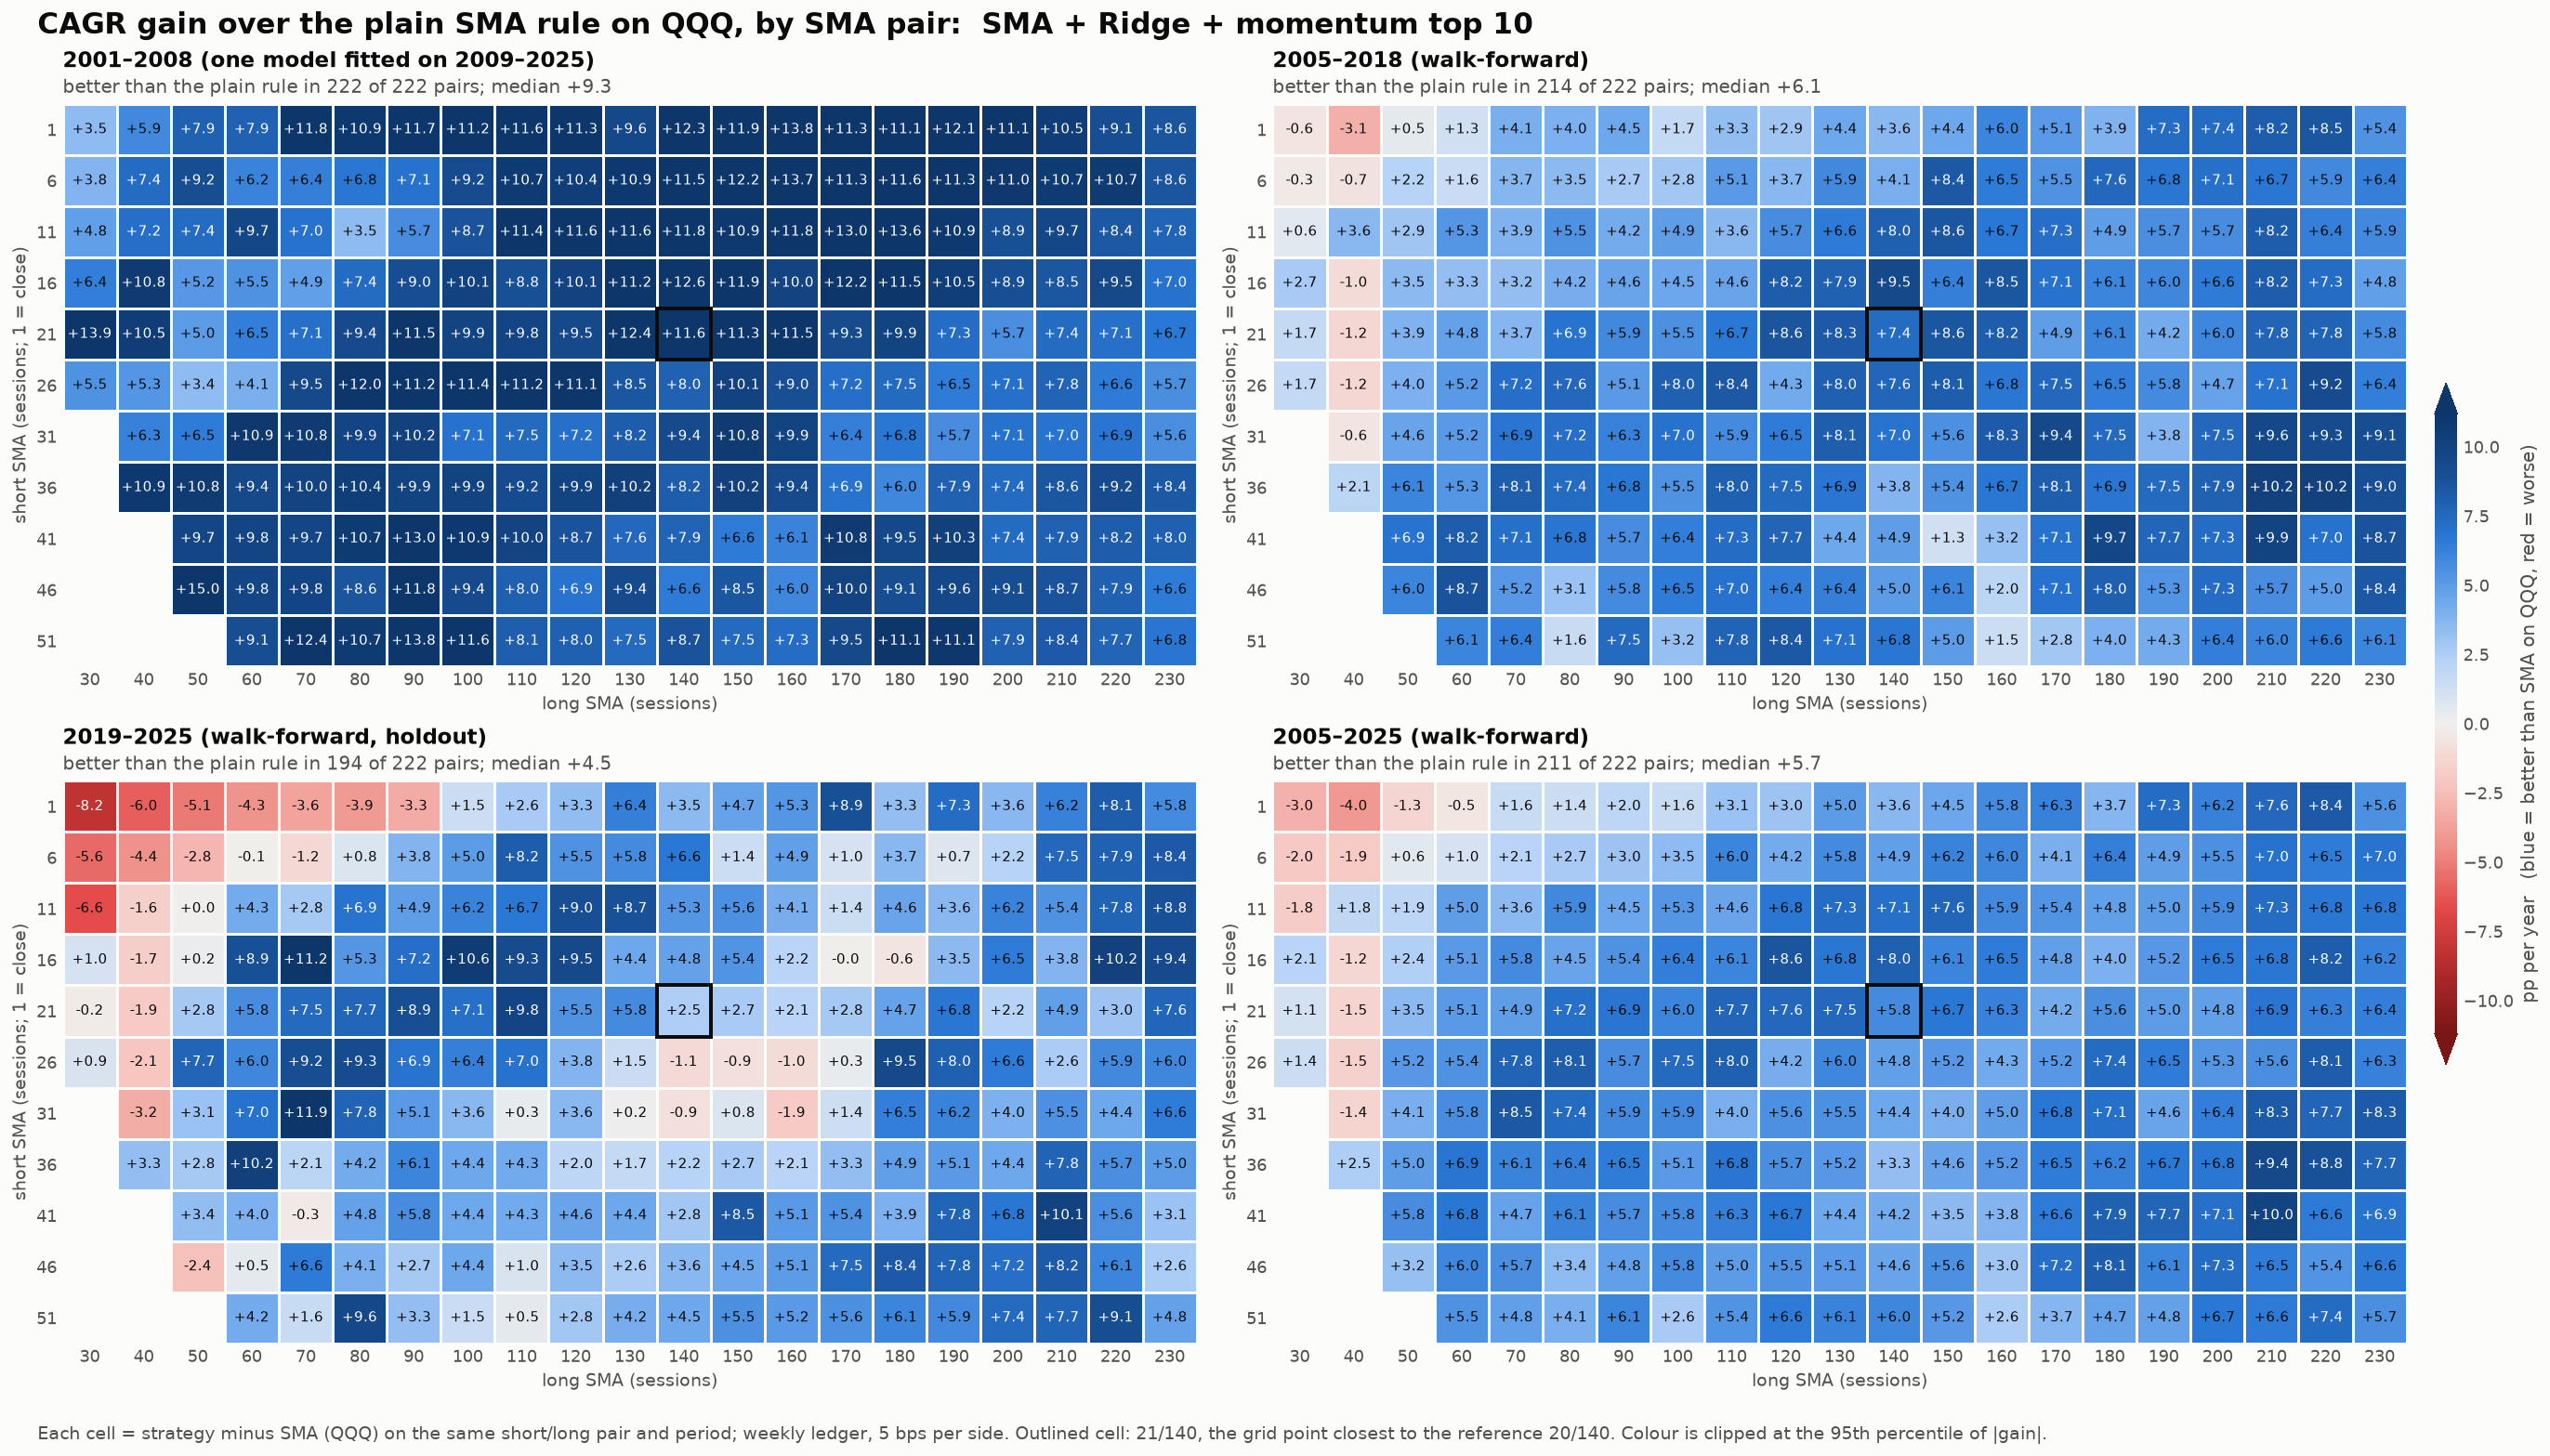
\includegraphics[width=\textheight,height=0.88\textwidth,keepaspectratio]{figures/figA3_walkforward_cagr.png}
\caption{Annual walk-forward and reverse-time test: CAGR gain of the three-component strategy (top ten) over the plain SMA rule.}
\label{fig:a3}
\source{\texttt{results/ablation/sma\_grid/}}
\end{sidewaysfigure}

\end{document}
